
\documentclass[12pt]{article}

\usepackage[latin1]{inputenc}
\usepackage{amssymb}
\usepackage{amsmath}
\usepackage{amscd}
\usepackage{amsthm}
\usepackage{amsfonts}
\usepackage{enumerate}
\usepackage{graphicx}
\usepackage{framed}
\usepackage{url}
\usepackage{amssymb}
%\usepackage[dvips]{color}
\usepackage{epsfig}
\usepackage{mathrsfs}
\usepackage{comment}
\usepackage{hyperref}

\usepackage{tikz}
\usetikzlibrary{arrows}


\pdfpagewidth 8.5in
\pdfpageheight 11in
\topmargin -1in
\headheight 0in
\headsep 0in
\textheight 8.5in
\textwidth 6.5in
\oddsidemargin 0in
\evensidemargin 0in
\headheight 75pt
\headsep 0in
\footskip .75in


\newenvironment{ee}{\begin{enumerate}}{\end{enumerate}}
\newenvironment{ii}{\begin{itemize}}{\end{itemize}}

\newcommand{\argmax}{\arg\!\max}
\newcommand{\argmin}{\arg\!\min}

\newcommand{\abs}[1]{\left\vert #1 \right\vert}
\newcommand{\Var}{\text{Var}}
\newcommand{\Cov}{\text{Cov}}
\renewcommand{\Pr}[2]{\mathop{\text{Pr}}_{#1} \left[ #2 \right]}

\def\RR{\mathbb R}
\def\CC{\mathbb C}
\def\QQ{\mathbb Q}
\def\ZZ{\mathbb Z}
\def\NN{\mathbb N}
\def\powset{\mathbb P}
\def\FF{\mathbb F}

\def\e{\epsilon}
\def\d{\delta}
\def\p{\partial}
\def\Chi{\chi}

\def\ds{\displaystyle}
\newcommand{\vs}[1]{\vspace{#1 pt}}

\def\tensor{\otimes}
\def\xor{\oplus}

\newcommand{\floor}[1]{\left\lfloor #1 \right\rfloor}
\newcommand{\ceil}[1]{\left\lceil #1 \right\rceil}
\newcommand{\field}[1]{\mathbb #1}
\newcommand{\inner}[2]{\langle #1,#2\, \rangle}
\newcommand{\norm}[2]{\| #1 \|_{#2}}
\newcommand{\ket}[1]{| #1 \rangle}
\newcommand{\bra}[1]{\langle #1 |}
\newcommand{\dirac}[2]{\langle #1 | #2\, \rangle}


\newcommand{\bracket}[1]{\langle #1 \rangle}
\newcommand{\paren}[1]{\left( #1 \right)}
\newcommand{\set}[1]{\left\{ #1 \right\}}

\newcommand{\bset}{\left\{0,1\right\}}

\newcommand{\inv}{^{-1}}
\newcommand{\til}{\widetilde}
\newcommand{\sign}{\mathrm{sgn}\;}
\renewcommand{\mod}{\text{ mod }}

\newcommand{\poly}{\text{poly}}
\newcommand{\polylog}{\text{polylog}}
\newcommand{\tsc}[1]{\textsc{#1}}
\newcommand{\tmc}[1]{\mathcal{#1}}

\newcommand{\Co}{{\sf Co-}}
\newcommand{\co}{{\sf co}}
\newcommand{\modpoly}{/ \text{poly}}
\newcommand{\SPACE}{{\sf SPACE}}
\newcommand{\TIME}{{\sf TIME}}
\def\D{{\sf D}}
\def\N{{\sf N}}
\def\P{{\sf P}}
\def\L{{\sf L}}
\def\E{{\sf E}}
\newcommand{\promise}{\textsf{promise}}

\newcommand{\NP}{{\sf NP}}
\newcommand{\PSPACE}{{\sf PSPACE}}
\newcommand{\EXP}{{\sf EXP}}

\newcommand{\BP}{{\sf BP}}

\newcommand{\NL}{{\sf NL}}

\newcommand{\NC}{{\sf NC}}
\newcommand{\AC}{{\sf AC}}
\newcommand{\RP}{{\sf RP}}
\newcommand{\BPP}{{\sf BPP}}
\newcommand{\PH}{{\sf PH}}
\newcommand{\PP}{{\sf PP}}
\newcommand{\IP}{{\sf IP}}
\newcommand{\AM}{{\sf AM}}
\newcommand{\MA}{{\sf MA}}
\newcommand{\PCP}{{\sf PCP}}

\newcommand{\FO}{{\sf PA}}
\newcommand{\SO}{{\sf PA}}
\newcommand{\PA}{{\sf PA}}
\newcommand{\ZF}{{\sf ZF}}
\newcommand{\ZFC}{{\sf ZFC}}

\newtheorem{theorem}{Theorem}[section]
\newtheorem{lemma}[theorem]{Lemma}
\newtheorem{proposition}[theorem]{Proposition}
\newtheorem{prop}[theorem]{Proposition}
\newtheorem{corollary}[theorem]{Corollary}
\newtheorem{conjecture}[theorem]{Conjecture}

%\theoremstyle{definition}
\newtheorem{example}[theorem]{Example}
\newtheorem{problem}[theorem]{Problem}
\newtheorem{definition}[theorem]{Definition}
\newtheorem{question}[theorem]{Question}
%\theoremstyle{remark}

\newtheorem{remark}[theorem]{Remark}
\numberwithin{equation}{section}

\renewcommand{\theequation}{\thesection.\arabic{equation}}




\begin{document}

\title{{\bf Efficient Inference in Probabilistic Computing} \\ M.Eng Thesis}
\author{Jeff Wu \\ \\ {\small Advised by Vikash Mansinghka and Josh Tenenbaum}}
%\address{}
%\email{}
\date{}
\maketitle
%
%\begin{center} \begin{LARGE} {\sc \bf Title} \vs{6}

%{\sc M.Eng Proposal} \vs{9}

%\end{LARGE} { \Large \textsc{Jeff Wu}}

%\end{center}

%\begin{abstract}
%\end{abstract}





%TITLE: Saving Memory and Time in Church Inference via Reduced Traces and Just-in-Time Compilation
%
%ABSTRACT
%
%INTRODUCTION
%
%[[FIXME outline]]
%
%[[FIXME Schematic of complexities]]
%
%Figure 1. {\bf Different Church architectures exhibit different predictable time, space and entropy costs per iteration of the inference Markov chain.} [[FIXME expand]]
%
%Figure 2. {\bf An illustration of full versus reduced computation traces.}  [[FIXME explain]]
%
%Figure 3. {\bf Computation traces captured from our Python implementation.} {\em (top)} A full computation trace for the [[FIXME]] program. {\em (bottom)} A reduced computation trace; these have far fewer nodes and far sparser dependencies than full traces.
%
%Figure 4: {\bf Just-in-time compilation using the RPython tracing JIT generator.} {\em (top)} The dataflow of a tracing JIT [[FIXME expand]] {\em (middle)} The software architecture of our tracing JIT based inference engine. {\em (right)} 
%
%Figure 5: {\bf The time and space complexities of full and reduced traces, with and without JITting, on a range of illustrative probabilistic programs.} {\em (A)} A categorical sampler implemented via a recursion within Church involves a a large number of deterministic recursions. [[FIXME cateogircal ;BN; topic; crp mixture]]
%
%Figure 6: {\bf Topic models.} [[FIXME]]

\tableofcontents{}

\section{Introduction}


Probabilistic programming languages are generalizations of programming languages, in which procedures are replaced with random procedures that induce distributions.  By allowing for easy description and manipulation of distributions, probabilistic programming languages let one describe classical AI models in compact ways, and provide a language for very richer expression.  

A core operation of probabilistic programming languages is inference, which is a difficult computational problem in general\cite{Dagum}.  However, Markov chain Monte Carlo (MCMC) methods converge quite quickly to the posterior distribution for a large class of inference problems.  Much effort has been devoted to studying in which cases this inference is efficient, and how to make it so.  \\

We explore implementations of a programming language much like Church \cite{Goodman}.  A naive implementation of inference uses a database to store all random choices \cite{lightweight}, and re-performs all computations on each transition.  

To improve this, we introduce a ``traces" data structure, letting us represent the program structure in a way that allows us to do minimal re-computation.  During inference, we make one small change and propagate the changes locally. 

Unfortunately, the trace structure takes up significantly more space than the random database.  Thus we introduce ``reduced traces", which takes the same amount of space (asymptotically) as the random database.  While it is asymptotically slower than traces for some programs, we demonstrate that the time complexity is similar in practice.  \\

We also remark on another significant advantage of reduced traces.  While writing interpreters in Python is typically considered slow, the PyPy translation toolchain aims to let developers compile their interpreters into lower level languages, such as C.  %, so long as they write their code in a restricted version of Python called RPython.  
Furthermore, one can use various hints to generate a tracing JIT.  Generating a tracing JIT for inference could potentially improve efficiency greatly, and reduced traces make this far easier to implement. \\

Thus far, in this project, we have done the following:
\begin{enumerate}
\item Explore the theoretical aspects of the traces and reduced traces inference algorithms.
\item Implement the different inference engines, in RPython, so as to have C versions of the interpreter.  All engines conform to a common REST API.  \footnote{Server code here:  https://github.com/WuTheFWasThat/Church-interpreter}
\item Run various benchmarks on the engines to compare the engines' performance on various problems. % Demonstrate good performance on a large-scale topic model!  % Apply the engine to a real-world problem, recovering classic algorithms for topic modeling to demonstrate efficiency.
\end{enumerate}
There are many research directions to pursue after this, all towards the goal of improving performance of the inference engine:
\begin{enumerate}
\item Generate a tracing JIT version of the interpreter.
\item Creating a parallelized version of reduced traces.
\item Potentially exploring some ``adaptive" generalizations of Gibbs sampling.
\end{enumerate}

We would ultimately like to recover the efficiency of special-cased inference algorithms for topic-modeling, mixture modeling, and Hidden Markov Models, in a much more general setting, and with far fewer lines of code.

% introduction: restate goals from above, of course including which research direction (parallelism; noise variables; connections to deterministic algorithms like sorting) we actually did


%INTRO
%build pcp engine which i understand well
%tested on variety of problems
%study tractability of inference on other harder problems
%do performance engineering / parallelism

%write-up spec of language
%write-up test cases

%write mixture-model

%\subsection{Outline}

%In this paper, we first give an overview of our language and its implementation.  



\section{Language description}

\begin{comment}

\subsection{Values}

A {\bf value} is a valid binding for a variable, in our language.  For example, integers, floats, and booleans are valid values.  We call these primitive values.  Another type of value is a {\bf procedure}, a function which gets applied to arguments and returns (not necessarily primitive) values.  

These procedures should be non-deterministic.  To allow for this, we can imagine that there is a special procedure, call it {\tt bernoulli}, which takes an argument $p$, and outputs 0 or 1, with probabilities $1-p$ and $p$, respectively.  Arbitrary random procedures can then be built up using this one.   We will see later that we actually can and will allow for something far more general than random procedures.

%Suppose I declare in some program that {\tt x} is determined by a coin flip.  But on any given execution of the program, {\tt x} must take on one of two values.  \vspace{6 pt}


\subsection{Expressions and Environments}

{\bf Expressions} are syntactic building blocks, which specified as being one of the following:
\begin{itemize}
\item Atomic expressions:
\begin{itemize}
\item A value itself.
\item A variable name.
\end{itemize}
\item Non-atomic expressions
\begin{itemize}
\item An application of an expression to a list of argument expressions.
\item A function, consisting of some variable arguments, and a body expression.
\item An if statement, consisting of a branching expression, and two child expressions.
\item An operator statement, consisting of an operator (e.g. == , $<$ , + , $\times$ , {\tt AND}, {\tt OR}, {\tt NOT}) and a list of argument expressions.
% \item A switch statement, consisting of a branching expression, and a list of child expressions
% \item A let statement
\end{itemize}
\end{itemize}

Expressions are {\bf evaluated}, so that they take on some value.  Their evaluation is relative to an {\bf environment}, in which variable names may be bound to values.  

Evaluation happens recursively.  If an invalid expression is ever given (e.g. the first expression in an application isn't a procedure, or we call the equality operator with three arguments), an error is thrown.  

\end{comment}

\subsection{Values and expressions}


A {\bf value} is a valid binding for a variable, in our language.  For example, integers, floats, and booleans are valid values.  We call these primitive values.  Another type of value is a {\bf procedure}, a function which gets applied to a tuple of argument values and returns another value.  These procedures may, of course, be non-deterministic.  

Our language contains some default procedures, from which we can then build up more complicated ones.  In fact, as we all see later, the types of procedures we allow will end up being more general than that which is typically thought of as a procedure.  \\

{\bf Expressions} are syntactic building blocks.  % Please refer to \cite{Goodman} for more details. 
Expressions are {\bf evaluated}, so that they take on some value.  Their evaluation is relative to an {\bf environment}, in which variable names may be bound to values.   All expressions are one of the following: % (the syntax is much like Scheme)

\begin{itemize}
\item A name, e.g. x or y, which refers to a value bound in the current environment.
\item A constant value, e.g. $3$, $3.1415$, True, or a default procedure.
\item A lambda expression, i.e. $(\lambda \  (x_1 \ldots x_n) \ \text{body\_expression})$, which evaluates to a procedure taking $n$ arguments.
\item An application, i.e. $(f \ x_1 \ x_2 \ \ldots \ x_n)$, where $f$ is a procedure taking $n$ arguments.
\end{itemize}

\subsection{Directives}

There are three basic operations, called {\bf directives}, which the language supports.  They are:

\begin{itemize}
\item {\tt PREDICT [expr]} 

Evaluates with respect to the global environment to sample a value for the expression {\tt expr}.

\item {\tt ASSUME [name] [expr]} 

Predicts a value for the expression {\tt expr}, and then binds {\tt name}, a string variable name, to the resulting value in the global environment.

\item {\tt OBSERVE [expr] [val]} 

Observes the expression {\tt expr} to have been evaluated to the value {\tt val}.  Runs of the program should now be conditioned on the expression evaluating to the value.
\end{itemize}

\noindent There are many other commands.  But by far the most interesting and important one is inference.
\begin{itemize}
\item {\tt INFER [rerun] [iters]} 

Runs {\tt iters} steps of the Markov Chain, also deciding whether to first rerun the entire program.  The result of running sufficiently many iterations from the prior, should be that sampling gives the posterior distribution for expressions, conditioned on all the observed values.  Restarting from the prior will not be typically used, but is useful for performance comparisons.

\end{itemize}

\noindent Other commands do various useful things like report various benchmarks (including time, space, and entropy use), help us gather statistics, allow seeding of the underlying PRNG, and deleting parts of the program or clearing it entirely.  
%The {\tt observe} primitive is required to be 



\section{Inference}

Inference is by far the most complicated of the directives, and also the most important.  Performing inference is the reason we are interested in probabilistic programming languages in the first place.  

% if we observe(blah, true), observe(blah, false)

%    - language definition with examples
%                - XRPs: what they are, and how to add them


%
%        - test cases. for each test case, include:

%            - a couple paragraphs and a figure explaining the purpose of the test
%                - analytical calculations or invariants showing what you'd expect if the interpreter was behaving correctly
%                - code for the program
%                - results, compared to the analytical section

%\subsection{Architecture of inference}

\subsection{First try}

Of course, the most obvious way to implement inference is to use rejection sampling.   But this scales poorly with the number of observations.  We'd like to instead run Metropolis-Hastings on the space of all possible executions of the program.  \\

Our proposal density, which chooses the new state (program execution history) to potentially transition to, does the following:   
\begin{enumerate}
\item Pick, at random, one of the random choices made, at any point in the program's execution history.  Make a new choice for this randomness.  
\item Rerun the entire program, changing only this choice.  If this causes us to evaluate new sections of the code (e.g. a different side of an if statement, or a procedure called with different arguments) with new choices of randomness, simply run these new sections freshly.  
%Also ``unevaluate" the evaluation of previously-evaluated sections which are no longer evaluated.   
% \item For all observations, use the outermost noise to force.  
\end{enumerate}

We then use the update rule of Metropolis-Hastings to decide whether we enter this new state, or whether we keep the old one.  However, if the new execution history doesn't agree with our observations, we assign it a probability of 0, so that we never transition to such a state.   

\subsection{Adding noise to observations}

Unfortunately, as it has been described, this random walk doesn't converge to the posterior!  Consider the following example, in which I flip two weighted coins and observe that they came up the same:  

\begin{leftbar} \begin{small} \begin{verbatim}
ASSUME a (bernoulli 0.5)
ASSUME b (bernoulli 0.5)
ASSUME c (^ a b)
OBSERVE c True 
\end{verbatim} \end{small} \end{leftbar}

It is easy to verify that the posterior distribution should have the state {\tt \{a:True, b:True\}} with probability $\frac{1}{2}$ and {\tt \{a:True, b:True\}} with probability $\frac{1}{2}$.  However, we can see that if we start in the state {\tt \{a:True, b:True\}}, we will never walk to either of the two adjacent states {\tt \{a:False, b:True\}} and {\tt \{a:True, b:False\}}.  So the random walk stays in the initial state forever!  The same argument applies if we start from {\tt \{a:False, b:False\}}.  Thus this Markov chain does not mix properly.  \vspace{6 pt}

To fix this problem, we should allow some small probability of transitioning to states where observations are false.  After all, a Bayesian should never trust their eyes 100\%!   Suppose instead of

\begin{leftbar} \begin{small} \begin{verbatim}
OBSERVE [expr] [val]
\end{verbatim} \end{small} \end{leftbar}

we instead used:

\begin{leftbar} \begin{small} \begin{verbatim}
OBSERVE (bernoulli (if (= [expr] [val]) 0.999 0.001)) True
\end{verbatim} \end{small} \end{leftbar}


Now, when we run our walk, if the expression {\tt (= [expr] [val])} evaluates to {\tt False} (so the original observation would've failed), we force the outermost {\tt bernoulli} application to be {\tt True}.   If the noise level is small, this should not affect results much, since the execution histories in which the original observation was false are weighted against heavily.  However, the space of states is always connected in the random walk and our Markov chain will converge properly.\vspace{6 pt}% I don't know if there is any formal sense in which this is really true...

For convenience, our language uses the function {\tt (noisy [observation] [noise])} as syntactic sugar for 
{\tt (bernoulli (if [observation] (- 1 [noise]) [noise]))}, where you have observed some expression {\tt [observation]} to be true.  

\subsection{A short example}

Let's start with a simple example, to get familiar with our language.   We will see how easy it is to write simple Bayes' nets, in our language (and in fact, it is easy to write much larger ones as well).

\begin{leftbar} \begin{small} \begin{verbatim}
>>> ASSUME cloudy (bernoulli 0.5)
id: 1
value: True
>>> ASSUME sprinkler (if cloudy (bernoulli 0.1) (bernoulli 0.5))
id: 2
value: False
\end{verbatim} \end{small} \end{leftbar}

Initially, we have this model, and we know nothing else.  So our prior tells us that there's a 30\% chance the sprinkler is on.

\begin{leftbar} \begin{small} \begin{verbatim}
>>> INFER sprinkler 10000 10
False: 6957
True: 3043
\end{verbatim} \end{small} \end{leftbar}

\noindent We now look outside, and see that the sprinkler is in fact on.  We're 99.9\% sure that our eyes aren't tricking us.  

\begin{leftbar} \begin{small} \begin{verbatim}
>>> OBSERVE (noisy sprinkler .001) True
id: 3
\end{verbatim} \end{small} \end{leftbar}

\noindent Now, we haven't yet looked at the sky, but we have inferred something about the weather.  

\begin{leftbar} \begin{small} \begin{verbatim}
>>> INFER cloudy 10000 10
False: 8353
True: 1647
\end{verbatim} \end{small} \end{leftbar}

This is quite close to the correct value of $\frac{5}{6} = 0.8\overline{333}$ False, which is what we'd get if there was no noise in our observation.  However, there is still a number of worlds in which the sprinkler was actually on.  In those worlds, the weather was more likely to be cloudy.  So we should expect error on the order of 0.001, but more error comes from our small sample size.  \vspace{6 pt}

\section{XRPs and Mem}

Up until now, we have neglected to mention a crucial aspect of our language.  The procedures allowed in our language are much more general than what we typically think of as procedures.  In this section, we introduce the most general type of procedures we can allow inference over.  

\subsection{Exchangeability}

Evaluating and unevaluating sections of code is very easy when all random choices are made independently of one another.  But actually, it is easy to evaluate and unevaluate so long as the sequence of random choices is {\bf exchangeable sequence}, meaning, roughly speaking, that the probability of some set of outcomes does not depend on the order of the outcomes.  In particular, as long as it is safe to pretend that the section of code we're unevaluating was the last section of code evaluated, we're fine!  %For a formal definition, see  \cite{}.

Thus instead of merely being able to flip independent coins as a source of randomness for procedures, the most general thing we are able to allow what is called an {\bf exchangeable random procedure (XRP)}.  An XRP is a type of random procedure, but different applications of it are not guaranteed to be independent; they are guaranteed merely to be an exchangeable sequence.  That is, the sequence of {\tt (arguments, result)} tuples is exchangeable.  The probability of a sequence is independent of its order (assuming we got the arguments in that order).\\

For example, if $f$ is an XRP taking one argument, we may find that $f(1) = 3$, and later that $f(2) = 4$.  Unlike a typical procedure, the result $f(2) = 4$ was not necessarily independent from the earlier result $f(1) = 3$.  However, the probability that this execution history happens should be the same as the probability that we first apply $f(2)$ and get $4$, and then later apply $f(1)$ and get $3$.  Of course, $f(2)$ can be replaced with $f(1)$ everywhere in this paragraph, as well --- multiple applications to the same arguments can also be different and non-independent, so long as they are exchangeable.

% We can see why this exchangeability condition still lets us do inference.  During inference, we want to reflip random choices from earlier in the program, while being able to preserve later choices.  Exchangeability lets us do precisely that, at no cost.  We can pretend the XRP application in question was the most recent one, and thus we can safely remove the value.  

\subsubsection{Formally specifying XRPs}

XRPs used in our probabilistic programs are specified by the following four functions:

\begin{itemize}
\item {\tt initialize()}, which returns an initial state.  
\item {\tt apply(state, args)}, which returns a value.
\item {\tt incorporate(state, value, args)}, which returns a new state.
\item {\tt remove(state, value, args)}, which returns a new state.
\item {\tt prob(state, value, args)}, which returns the (log) probability of returning the value, if the XRP in its current state is applied to the arguments.
\end{itemize}

The state of the XRP is a sufficient state, meaning it alone lets you determine the XRP's behavior.  Minimally, the state may be a history of all previous applications of the XRP, although in most cases, it is much more succinct.  Whenever we apply the XRP, we use {\tt apply} to determine the resulting value, and we may use {\tt prob} to determine the probability that we got that value, conditioning on all previous applications.  This value can then incorporated into the XRP using {\tt incorporate}, and the state is updated.  Finally, {\tt remove} lets you remove a value, undoing an incorporate.

Notice that if applications are independent, then we do not need a state, and both incorporate and remove can do nothing.  Thus this recovers the special case of normal random procedures.  

% However, for the remainder of the paper, we will use XRP to refer to procedures which are strictly non-deterministic.  All XRPs which are deterministic can simply be viewed as ordinary procedures. \\

XRPs are quite a general object, and replacing random procedures with them significantly increase the expressive power of our language.   They also come in a variety of flavors, and we will see some examples later.   % Of course, we now allow defining procedures which use and return other XRPs, since XRPs are valid values.  \\

\subsubsection{Re-apply or re-score}

If our XRP is capable of returning any value in its range, regardless of its arguments, then we will say it is a ``rescoring" XRP.  That is, if we are dynamically changing the program, and the XRP is passed new arguments but wants to retain its old value, we can do so, but perhaps with a modification to the probability.  

If our XRP is not capable of this, we call it a ``reapplying" XRP.  That is, it should reapply these new arguments to get a new value as well.

Essentially, in inference, when values change, and we are propagating the changes upwards, reapplying XRPs will ``pass on" the changes, whereas rescoring XRPs will ``absorb" them.  \\

Now, we can allow for something much more general than the noisy observations above.  We now simply require that all observed expressions have an outermost rescoring/absorbing XRP application.  When running inference, we always force the XRP to give the observed value by using {\tt inc} (without using {\tt apply}).  The probability of getting this observed value should always be non-zero.  
% Suppose that I observe that the sky is pink, and also that the ocean is yellow.  Chances are, either my vision has gone crazy, or the world has underwent drastic changes.  The correctness of my observations is highly correlated, and so we should allow for non-independent noise.  Luckily, XRPs allow for this.  

The noisy expressions obtained with {\tt noisy} are a special case of this, so long as {\tt noise} was non-zero.  

Also, notice that we could make all XRPs re-scorers, by adding noise to their output.  That is, we could have all XRPs have an internal error rate, as if {\tt noisy} were being applied.  

\subsection{Mem}

A special XRP worth noting is {\tt mem}, which lets us memorize procedures.  Applying {\tt mem} to a procedure returns another XRP, which is a memoized form of that procedure.  That is, when using a {\tt mem}'d procedure, we never reapply randomness, given old arguments.  Thus whenever we apply the memoized procedure once to some particular arguments, applying it again to those arguments will result in the same value. 

Implementation of {\tt mem} is extremely tricky, and we will decline to work out its details in this paper.  However, it is important to understand its utility.  As a simple example, consider a naive implementation of Fibonacci:


\begin{leftbar} \begin{small} \begin{verbatim}
ASSUME fib (lambda (x) (if (< x 2) 1 (+ (fib (- x 1)) (fib (- x 2)))))
\end{verbatim} \end{small} \end{leftbar}


\noindent Of course, evaluating fibonacci in this manner is an exponential time operation.  Evaluating {\tt (fib 20)} took nearly 2 seconds.  \\

Simply wrapping a {\tt mem} around the lambda expression will make it so we don't need to recompute {\tt (fib 20)} the next time we call it.  Not only that, but when we recurse, we will only compute {\tt (fib [x])} once, for each $x =0, \ldots, 20$.  

\begin{leftbar} \begin{small} \begin{verbatim}
ASSUME fib (mem (lambda (x) (if (< x 2) 1 (+ (fib (- x 1)) (fib (- x 2))))))
\end{verbatim} \end{small} \end{leftbar}


Evaluating {\tt (fib 20)} now takes well less than a millisecond. \\

One limitation of mem is that if the procedure argument to mem changes, the memorization must be reapplied.  unless mem is noisy, it needs to be reapplied. state that we could make a noisy-mem which takes a noise proc that is applied after the procedure is looked up each time.

\section{Traces}

The random database implementation of inference is not very interesting.  The inference engine simply reruns the program after each iteration, remembering all previous randomness chocies, and having only one choice changed.    Let's skip to the ``traces" implementation.


\subsection{Basic overview}

In the traces implementation of inference, we create an {\bf evaluation node} for every expression that is evaluated, which keeps track of the expression, environment, values, and many other things.  

The evaluation nodes are connected in a directed graph structure, via dependencies.  Thus if the evaluation of one node, $x$, depends on the evaluation of another (e.g. a subexpression, or a variable lookup), $y$, we say that $y$ is a {\bf child} of $x$ and that $x$ is a {\bf parent} of $y$.  By interpreting these child-parent relationships as edges (from parent to child), these evaluation nodes form a directed acyclic graph, which we refer to as the {\bf trace}.  

Each node caches the relative locations and values of all its children.  Furthermore, if it is an application node, we also cache the procedure and arguments.  And for every node, we cache its most recent value.  

%\subsection{The proposal}
%
%When we re-flip the value of some XRP application, we would like to simply remove the old value, and then incorporate a new value directly, asking for the probabilities as we do so, in order to calculate the MH ratio.  This appears to be valid, by the exchangeability property.  
%
%We'd then like to propagate the new value throughout the trace, by repeatedly propagating new values to parents.   If we reach a ``re-scoring" XRP application, we simply reuse its old value, so that we do not need to propagate computation any further (even if its arguments have changed).   If new branches need to be evaluated, it is done on demand.  
%
%However, how do we consider the probabilities of these other applications?  Unfortunately, the singular remove and then apply is only valid once.  We can't imagine multiple XRP applications to be the last one.  We can at best imagine $n$ applications to be the last $n$.  Thus, conceptually, we must remove all old values before applying and incorporating the new ones (and calculating their probabilities). \\
%
%Unfortunately, doing this would mean that we can't decide the values while we propagate up, and so we cannot stop propagating, even if the values are the same.  To fix this, we will use a different MH proposal.  
%
%Let's simply apply and incorporate all new values encountered, but refrain from removing the old values, and querying the probabilities as we go.  This will give us our ``forwards" transition probability the denominator of the MH ratio (with some cancelling).  Then, only at the end of our calculation, we can remove all old unused values, again getting the ``unevaluation" probabiltiies.  This determines our ``backwards" transition probability, or the numerator of the MH ratio (with some cancelling).  
%
%Let's outline more explicitly.  We will assume access to a global variable which will keep track of the probability of the current state.  Also, each node should keep track of whether it was forced
%% Using (if P C A) as an example.
%\begin{enumerate}
%\item Before the proposal: P = true, C is evaluated, A is not evaluated.    Global p = $P(X_{old})$ and number of unconstrained random choices is already known.
%\item Proposal.  A is being evaluated without removing things (sampled values from XRP application nodes) in C. Calculating $Q(X_{old} \rightarrow X_{new})$, not including constraint random choices. Update global p.
%\item Proposal is finished. Removing things in C. Calculating $Q(X_{new} \rightarrow X_{old})$, not including constraint random choices.
%\item $P(X_{new})$ and number of unconstrained random choices is now known. 
%\item Make MH decision basing on MH ratio.
%	\begin{itemize}
%\item PROPOSAL ACCEPTED: unsample and remove A, add C back.
%\item PROPOSAL REJECTED: unsample C.
%	\end{itemize}
%\end{enumerate}

% hash table with get random key
\subsection{Propagation}

How does propagation actually work?   This question is surprisingly interesting, and we explore two different candidate propagation schemes.

\subsubsection{Recursive propagation}

The easiest version of propagation to implement is simply a recursive, ``depth-first" implementation.  We simply start at the node which we reflipped, and recursively re-evaluate its parents, stopping only when we reach XRP application nodes.   However, notice that in a graph where nodes have multiple children and parents, this does not guarantee that we only propagate each node once.  In fact, this propagation has exponentially bad worst-case scenarios, and can be poor in some practical settings.  

Suppose we have the following program, which computes a familiar multivariate recurrence.

\begin{leftbar} \begin{small} \begin{verbatim}
ASSUME binom (lambda (n k) (if (or (= k 0) (= k n)) 1 
...                            (+ (binom (- n 1) (- k 1)) (binom (- n 1) k)))) 
\end{verbatim} \end{small} \end{leftbar}

Let's say we want to randomly replace one of the entry $n=2, k=1$ of Pascal's triangle with a random real number between 0 and 2.  And we are curious in the resulting distribution for the entry $n = 20, k = 10$. 

\begin{leftbar} \begin{small} \begin{verbatim}
ASSUME binom-wrong (lambda (n k c) (if (and (= n 2) (= k 1)) c (binom n k))) 
PREDICT (binom-wrong 20 10 (uniform-continuous 0 2))
\end{verbatim} \end{small} \end{leftbar}

\begin{center}
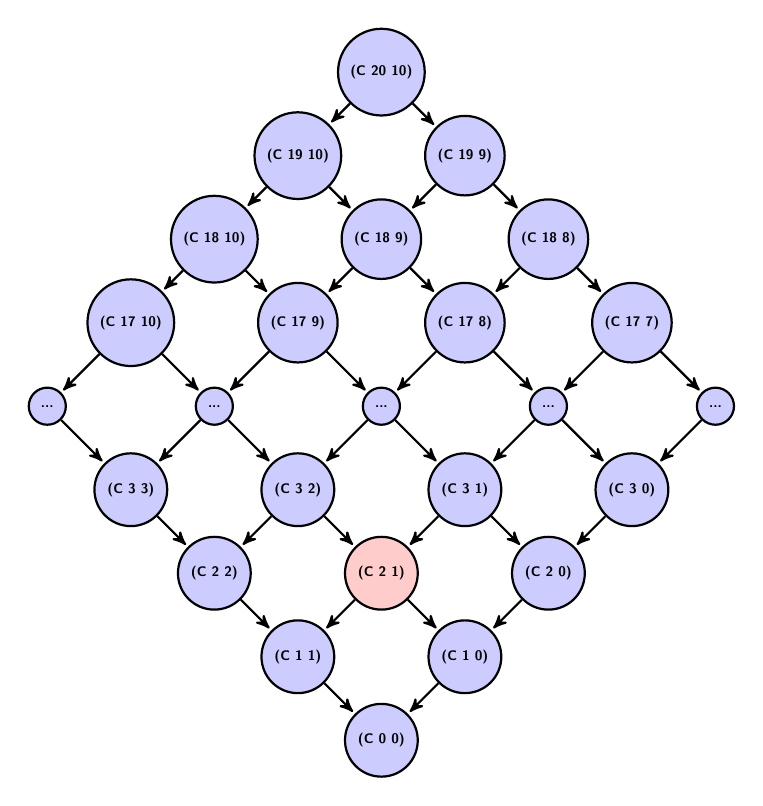
\begin{tikzpicture}[>=stealth',shorten >=1pt,auto,node distance=1.5cm,
  thick,main node/.style={circle,fill=blue!20,draw,font=\sffamily\tiny\bfseries}]

  \node[main node] (1) {(C 20 10)};
  
  \node[main node] (2) [below left of=1] {(C 19 10)};
  \node[main node] (3) [below right of=1] {(C 19 9)};
  
  \node[main node] (4) [below left of=2] {(C 18 10)};
  \node[main node] (5) [below right of=2] {(C 18 9)};
   \node[main node] (6) [below right of=3] {(C 18 8)};
   
     \node[main node] (7) [below left of=4] {(C 17 10)};
  \node[main node] (8) [below right of=4] {(C 17 9)};
   \node[main node] (9) [below right of=5] {(C 17 8)};
   \node[main node] (10) [below right of=6] {(C 17 7)};

     \node[main node] (11) [below left of=7] {...};
  \node[main node] (12) [below right of=7] {...};
   \node[main node] (13) [below right of=8] {...};
   \node[main node] (14) [below right of=9] {...};
   \node[main node] (15) [below right of=10] {...};
   
        \node[main node] (16) [below right of=11] {(C 3 3)};
  \node[main node] (17) [below right of=12] {(C 3 2)};
   \node[main node] (18) [below right of=13] {(C 3 1)};
   \node[main node] (19) [below right of=14] {(C 3 0)};

  \node[main node] (20) [below right of=16] {(C 2 2)};
  \node[main node] (21) [fill=red!20, below right of=17] {(C 2 1)};
   \node[main node] (22) [below right of=18] {(C 2 0)};
   
     \node[main node] (23) [below right of=20] {(C 1 1)};
  \node[main node] (24) [below right of=21] {(C 1 0)};
  
    \node[main node] (25) [below right of=23] {(C 0 0)};
    
\draw [->] (1) -- (2);
\draw [->] (1) -- (3);
\draw [->] (2) -- (4);
\draw [->] (2) -- (5);
\draw [->] (3) -- (5);
\draw [->] (3) -- (6);
\draw [->] (4) -- (7);
\draw [->] (4) -- (8);
\draw [->] (5) -- (8);
\draw [->] (5) -- (9);
\draw [->] (6) -- (9);
\draw [->] (6) -- (10);

\draw [->] (7) -- (11);
\draw [->] (7) -- (12);
\draw [->] (8) -- (12);
\draw [->] (8) -- (13);
\draw [->] (9) -- (13);
\draw [->] (9) -- (14);
\draw [->] (10) -- (14);
\draw [->] (10) -- (15);

\draw [->] (11) -- (16);
\draw [->] (12) -- (16);
\draw [->] (12) -- (17);
\draw [->] (13) -- (17);
\draw [->] (13) -- (18);
\draw [->] (14) -- (18);
\draw [->] (14) -- (19);
\draw [->] (15) -- (19);

\draw [->] (16) -- (20);
\draw [->] (17) -- (20);
\draw [->] (17) -- (21);
\draw [->] (18) -- (21);
\draw [->] (18) -- (22);
\draw [->] (19) -- (22);


\draw [->] (20) -- (23);
\draw [->] (21) -- (23);
\draw [->] (21) -- (24);
\draw [->] (22) -- (24);

\draw [->] (23) -- (25);
\draw [->] (24) -- (25);

\end{tikzpicture} \\
\begin{small} {Propagating from the red node upwards.  Here the C function is {\tt binom-wrong}.} \end{small}
\end{center}

Now suppose we decided to reflip the {\tt uniform-continuous} application.  And suppose we have the policy of always propagating to the right first, if possible.  We can then verify that the worst-case number of times we may propagate to the application {\tt (binom-wrong m l)} is essentially {\tt (binom m l)}.  \\

Intuitively, we wanted to propagate to the smaller values first, in this modified Pascal's triangle.  Then, we would only have needed to propagate about 100 times; once for each node.  Thus we see that the order is extremely important, in general.  

However, although the worst case scenario is terrible, this method of propagation is okay in practice for many problems.

\subsubsection{Full location}

So, we see is that the order of propagation is quite important.  How can we know which parents to propagate our values to first?   Intuitively, since our trace structure is a DAG, we simply propagate to those ``lowest" in the DAG.  Essentially, we want to maintain a priority queue, from which we will repeatedly remove the minimum and add his parents to the queue, until the queue is empty.  Here, we are simply interpreting the parent-child relationships as comparisons in a partial ordering.  


Unfortunately, a heap does not work correctly on a set of elements with only a partial ordering (even with ties arbitrarily broken), and so we must extend to some full ordering.  

We cannot simply use timestamps of the initial evaluation, since it is possible for unevaluated branches earlier in the program to be evaluated later.  

We could use a full description of the node's location (something like a call stack), but it would be quite expensive, %leading to asymptotic increases in both time and space.  
as comparisons would now take $O(h)$, where $h$ is the height of the DAG, defined to be the length of the longest directed path starting from a directive node.  %And each node would require $O(h)$ space, instead of $O(1)$ space.  Unfortunately, the story is somewhat worse than that.  Thus when evaluating the program itself, we also take a hit of $O(h)$.  

%\subsubsection{Partial location}
% 
%A final solution is to use a tuple, {\tt (directive-id, distance from directive node)}.  To decide whether to propagate to $x$ or to $y$, we first compare the directive they are immediately underneath.  We prefer to propagate to nodes with smaller id.  In case of a tie, we then look at distance from the node corresponding to the directive itself.  We prefer to propagate to nodes further from the directive.  
%
%By propagating this way, we ensure that we only do constant work for each node.  We do some work evaluating while propagating up, and we potentially do work unevaluating, if the branch becomes irrelevant (e.g. the predicate of an if statement changes).  \\
%
%We might hope that our solution results in the minimal amount of propagation needed, in general. However, this is false for at least some families of problems.  For example, consider the following code, where {\tt f} is some arbitrary deterministic function:
%
%\begin{leftbar} \begin{small} \begin{verbatim}
%ASSUME roll (uniform 1 6)
%ASSUME result (if (> roll 1)
%                  (if (> roll 2)
%                      (if (> roll 3) 
%                          (if (> roll 4) 
%                              (if (> roll 5)
%                                  (f 6) (f 5)) (f 4)) (f 3)) (f 2)) (f 1)) 
%\end{verbatim} \end{small} \end{leftbar}
%
%Suppose {\tt roll} is currently {\tt 6}, so that the branch at {\tt (f 6)} is currently active.  If we reflip the application of {\tt uniform} so that {\tt roll} becomes {\tt 1}, we might hope that the correct value is propagated to the outermost occurrence of {\tt roll}, so that we merely unevaluate the branch to {\tt (f 6)} and evaluate the branch to {\tt (f 1)}.  
%
%However, what happens in reality is different.  We first propagate to the lowest occurrence of {\tt roll}, which leads us to unevaluate {\tt (f 6)} and evaluate {\tt (f 5)}. We then propagate to the second lowest occurrence, which leads us to unevaluate {\tt (f 5)} and evaluate {\tt (f 4)}.  This continues, so that by the end of our reflipping, we have evaluated {\tt (f x)} for all {\tt x = 1, \ldots, 6}.  \\
%
%What we'd like to do is to make sure that the predicate of an if branch precedes the consequents.  We run into a similar problem when evaluating procedure applications, where we'd like to evaluate the arguments before the body.  However, to do these things appears to require using longer keys for comparison, and we recover the ``full location" method.  
%

\subsubsection{Analysis}

As described above, the trace is not static across different runs of the same program.  When referring to this dynamic data structure, we will say, the {\bf dynamic trace}.  We may think of the dynamic trace as a random variable, where the randomness is over the different runs of the program.  % Whenever we take expectations, the expectation will be over runs of the program.  

For every node $x$, we say the {\bf envelope} of $x$, denoted $V_x$, is the set of nodes reached by propagating upwards in the dynamic trace until we reach ``re-scoring" XRP application nodes (including the application nodes, as well as $x$), and then propagating down through the %consequents of any conditionals we pass through and the 
bodies of any procedure applications we pass through. % \footnote{The envelope should bear some resemblance to the notion of a Markov blanket.   Indeed, it captures some aspect of conditional independence.}  
We think of $V_x$ a random variable as well, but it is only defined over worlds in which node $x$ is active in the dynamic trace.  

Now let $p_x$ be the probability that node $x$ is chosen to be reflipped in the Markov chain.  In other words, $p_x$ should represent the distribution where, first, we sample from a run of the program, and then we pick one of the XRP applications uniformly at random.  Lastly, we let $V$ be the random variable which first picks some $x$ with probability $p_x$, and then picks a random $V_x$, conditioned on $x$ being active.

We then have that the expected propagation time of the ``full location" propagation scheme is 
$$E_V[ |V| \cdot h \log |V| | = h  \cdot E_V[|V| \log |V|]. $$

This essentially follows directly from our propagation algorithm.  We do just as much unevaluating as evaluating, but this introduces just a factor of 2.  

% Although we may evaluate new parts, outside of $V_x$, when choosing $x$, we can use amortized analysis to show this is okay; essentially, we evaluate this work as part of the next reflipping instead.  
 
%Branches of conditionals can be evaluated and unevaluated, as well as branches corresponding to procedure applications to specific arguments.   

%Let us now turn towards a different picture.  Though the trace may change structures, depending on the values at various nodes, let us imagine a static version of the graph, in which all branches of computation are active.  We call this the {\bf static trace}.  
%
%Let's pay special attention to application nodes, which correspond to the application of a procedure to some arguments.  We would like to consider the static trace to have a child for each argument, a child for the procedure, and {\em only a single child} for the body, even if the function is called with many different tuples of arguments, across different computation histories.   
%
%In a dynamic trace, there is indeed only one child corresponding to the body, but in a static trace, there is a subtlety.  If the structure of the body is known in advance, then we may essentially have only one child.  But occasionally, we may not even know, statically, the structure of the procedure which is being applied.  For example, the child for the procedure could have a branching if statement.  Thus we imagine the static trace to have one node for each possible structure of the procedure body.  
%
%Notice that this static trace graph is not necessarily finite; after all, the computation itself may not be guaranteed to terminate.  For example, the following simple program has an infinite static trace.
%
%\begin{leftbar} \begin{small} \begin{verbatim}
%ASSUME decay-rate (rand)
%ASSUME geometric (lambda (x) (if (bernoulli decay-rate) x (geometric (+ x 1))))
%ASSUME decay-time (geometric 0)
%\end{verbatim} \end{small} \end{leftbar}
%
%For every node $x$, we say the {\bf static envelope} of $x$, denoted $V^+_x$, is the set of nodes reached by propagating upwards in the static trace until we reach XRP application nodes (including the application nodes, as well as $x$), and then propagating down through the consequents of any conditionals we pass through and the bodies of any procedure applications we pass through.  Similarly, we let $V^+$ be the random variable which first picks some $x$ with probability $p_x$, and then picks a random $V^+_x$, conditioned on $x$ being active.
%


% So we then have that the expected propagation time of the ``partial location" propagation scheme is 
% $$ E_{V^+}[|V^+| \cdot \log |V^+|]. $$


\section{Reduced Traces}

\subsection{Motivation}

The major downside of the traces implementation is that it is not memory efficient.  The number of nodes stored is essentially proportional to the time it takes to compute the original program, since we keep a node for each expression evaluation.  \\

% naming with a rolling hash


To highlight this, consider the following program, which samples from the categorical distribution, which returns $i$ with probability $p_i$.   The distribution is represented by some procedure {\tt categorical-dist}, which takes an argument $i$ and returns $p_i$.  It is guaranteed that for some finite $n$, $\sum_{i = 0}^{n-1} p_i = 1$

\begin{leftbar} \begin{small} \begin{verbatim}
ASSUME sample-categorical-loop 
        (lambda (v i)
                (if (< v (categorical-dist i)) 
                    i 
                    (sample-categorical-loop 
                     (- v (categorical-dist i))
                     (+ i 1))))

ASSUME sample-categorical (lambda () 
                            (sample-categorical-loop (rand) 0)
\end{verbatim} \end{small} \end{leftbar}

Notice that using traces, we will create a node for each application of the sub-loop.  And yet it is clear that this space is un-needed.  We feed the function a single choice of randomness, and it creates up to $n$ nodes.  But if we were to reflip the application of {\tt rand}, we would need to re-evaluate the entire application again.  Thus if $n$ is large, this could be a phenomenal waste of space.  Supposing a loop like this were on the critical path of some program, we could be using a multiplicative factor of $O(n)$ more space.  

One solution is to ``collapse" this sampling into an XRP.  That is, we turn {\tt sample-categorical} into an XRP, since applications of it are independent, and thus exchangeable.  This is a useful idea which we will turn back to later, but this is clearly not a satisfactory solution in general.  

\subsection{Reducing the traces graph}

The idea of reduced traces is to essentially ``contract" all edges of deterministic computation in the traces graph.  Whenever we need to perform deterministic computation, we will simply recompute, instead of having nodes all along the way with cached values.  

In contracting all these edges, the only nodes which remain will be nodes corresponding to XRP applications, and nodes which correspond to directives \footnote{There are also nodes corresponding to applications of {\tt mem}.}. \\

One minor issue which comes up is the locating of child nodes.  We need to be able to recover a specific child node, if we perform the computation leading to what should be its evaluation.  We also need to be able to figure out the location of children to unevaluate.  The relative locations may be long, and we don't want to store them in memory.

In order to do this, we using a rolling hash on the ``stack", a list which pins down the relative location of a node within the computation.  This technique is also used in the random database implementation of the engine.

\subsection{Propagation in reduced traces}

% We'd like to use the propagate nearly the exact same way as the ``partial location" method, in reduced traces.   However, the granularity at which we propagate up is much greater now.  Whenever we re-evaluate a node, we re-perform all the deterministic computation along the way, downwards in the DAG of computation, before propagating up again.  \\

% Interestingly, we can see that we will avoid the problem which we saw earlier with the dice roll.  Because we evaluate expressions from top-to-bottom, we have taken care of that issue for free!\\

In reduced traces, we essentially have the same options as in regular traces.  We won't go into detail explaining again.  

However, we will pay a price for our lack of structure.  Let's consider the following program, which indexes into an array using the max of two samples from the categorical distribution from the last example:

\begin{leftbar} \begin{small} \begin{verbatim}
ASSUME categorical-sum (+ (sample-categorical) (sample-categorical)) 
\end{verbatim} \end{small} \end{leftbar}

Now, each time we reflip the coin at the bottom of some {\tt sample-categorical}, we must re-evaluate both applications of sample-categorical, in order to propagate up to {\tt x}'s value.  Even in the analysis given for the static traces, evaluating this second argument was not necessary.  \\

The structure of a reduced trace is different from that of the traces we saw in the previous section, and this can lead to drastically worse running time.  For example, consider the following trace structure:\\

\begin{center}
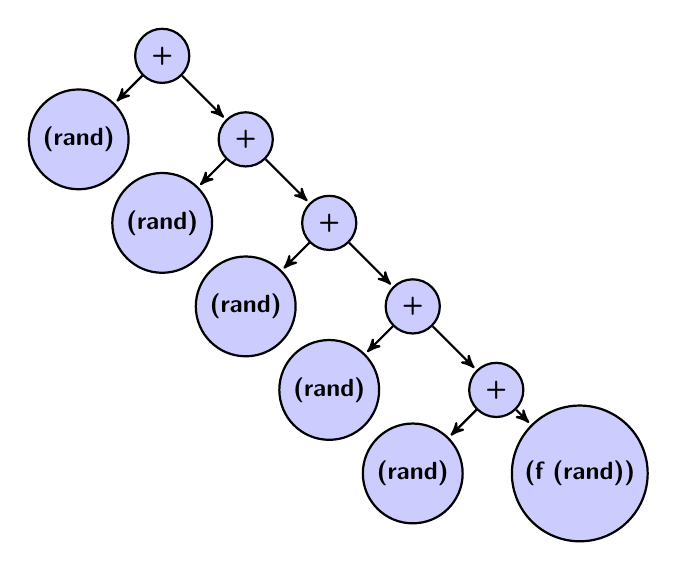
\begin{tikzpicture}[>=stealth',shorten >=1pt,auto,node distance=1.5cm,
  thick,main node/.style={circle,fill=blue!20,draw,font=\sffamily\small\bfseries}]

  \node[main node] (1) {+};
  \node[main node] (2) [below left of=1] {(rand)};
  \node[main node] (3) [below right of=1] {+};
  \node[main node] (4) [below left of=3] {(rand)};
  \node[main node] (5) [below right of=3] {+};
  \node[main node] (6) [below left of=5] {(rand)};
  \node[main node] (7) [below right of=5] {+};
  \node[main node] (8) [below left of=7] {(rand)};
  \node[main node] (9) [below right of=7] {+};
  \node[main node] (10) [below left of=9] {(rand)};
  \node[main node] (11) [below right of=9] {(f (rand))};
\draw [->] (1) -- (2);
\draw [->] (1) -- (3);
\draw [->] (3) -- (4);
\draw [->] (3) -- (5);
\draw [->] (5) -- (6);
\draw [->] (5) -- (7);
\draw [->] (7) -- (8);
\draw [->] (7) -- (9);
\draw [->] (9) -- (10);
\draw [->] (9) -- (11);
\end{tikzpicture}
\end{center}

Now suppose {\tt f} is an extremely expensive deterministic computation, so that the time it takes dominates all other runtime considerations.  In regular traces, we only need to recompute {\tt f} with probability 1 in 6, when its argument is reflipped.   However, in reduced traces, we must recompute it every time!  We no longer have values cached along the edges, and so we have traded in space complexity for some time complexity.

It's clear that we can generalize this example to a class of problems for which reduced traces does drastically worse.  However, as we will see, the runtime of reduced traces is empirically comparable to that of traces.  

\subsection{Analysis}

To analyze the propagation, we imagine we were still propagating in the old dynamic trace.  Although our notion of nodes is now different, we are really interested in the amount of computation done (essentially, number of expressions evaluated).  

Recall that we had defined the envelope to be the set of nodes reached by propagating upwards in a dynamic trace until we reached ``re-scoring" XRP application nodes, and then propagating down through % the consequents of any conditionals we passed through and 
the bodies of any procedure applications we passed through.  The set of nodes we evaluate is very similar, except that we additionally propagate downward from all other nodes with deterministic computation that we pass through, until we hit another application node (which has its value cached).  

Viewing the picture with only reduced traces, the set of nodes we propagate to is extremely analogous to the notion of Markov blankets, and also captures explicitly a notion of conditional independence.  

Let us call this set of nodes the {\bf full envelope}, $V^+_x$.  From the reduced trace point of view, we simply propagate to all parents, and then propagate down to their children which needed to be evaluated.  However, it is the set of nodes from the traces point of view that we are interested in.  

Again, we can consider the reduced trace to be dynamic, in this analysis, using the same sort of amortized analysis we had done earlier.  Thus the runtime is
$$ E_{V^+}[|V^+| \cdot \log |V^+], $$
where $V^+$ is the random variable which first picks some $x$ with probability $p_x$, and then picks a random full envelope $V^+_x$, conditioned on $x$ being active.

\subsection{Engine Complexity Trade-offs Summary}

To summarize, we have the following table of asymptotic complexities:

\begin{table}[h]
\caption{Engine Complexity Trade-offs} \label{sample-table}
\begin{center}
\begin{tabular}{c|c | c |c } % | c
& {\bf  Time / Iteration} & {\bf Space} & {\bf Time} \\ \hline % & {\bf h / iter}
{\bf Random DB} & $T$ & H + P & $T$\\  % & 1? 
{\bf Traces 1 (recursive)} & $E_V[2^V]$ & $T \ (\, + \ H + P)$ & $T$ \\ % & H(site)
{\bf Traces 2 (full location)} & $h \cdot E_V[V \log V]$ & $T \ (\, + \ H + P)$  & $h \cdot T$\\ % & H(site)
%{\bf Traces 3 (partial location)} & $E_{V^+}[V^+ \log V^+]$ & $T \ (\, + \ H + P)$ & $T$ \\ % & H(site)
{\bf Reduced Traces (recursive)} & $E_{V^+}[2^{V^+}]$ & H + P& $T$\\ % & H(site) 
{\bf Reduced Traces (full location)} & $E_{V^+}[V^+ \log V^+]$ & H + P& $T$\\ % & H(site)  %  \footnote{There are some additional costs, due to storing environments, and {\tt mem}. }
\end{tabular}
\end{center}
\end{table}

Here, the variables mean the following:
\begin{itemize}
\item $P$ = Size of the program description (the directives and their expressions)

\item $T$ = Expected runtime of the original program 

\item $H$ = Expected entropy (number of XRPs)

\item $V$ = Envelope size, in dynamic trace

\item $V^+$ = Full envelope size, in dynamic reduced trace

\item $h$ = The ``height" of the program.  That is, the largest number of evaluations any node is away from a directive.
\end{itemize}

Recall that $T > H$ and $T > P$, and $V < V^+$. \\ % and $V > F$.  \\

Though none of the traces implementation is strictly dominated by another, we believe the 1st and especially 3rd are more likely to be efficient in practice.  And we believe that reduced traces should have much better space usage and only marginally worse run-time.  See the appendix for some preliminary empirical results.

\section{Extended XRPs}

We now discuss some extensions to the XRP interface, to give the user more power over how inference works.  

\subsection{XRP weights}

By default, all XRP applications are equally likely to be reflipped.  But what if we would like to reflip some XRP applications more than others?  This won't affect the resulting distribution, so long as we correctly calculate transition probabilities, but it could be helpful for making our chain mix much faster.  

To achieve this, we will assign each XRP a weight, which tells us how often we should reflip its applications, relative to other ones.  This is extremely useful for certain programs.  % For example, one might want to assign XRP applications a weight which reflects the number of possible values it could take on.  
However, in order to use this, we'd like a data structure supporting the following operations:

\begin{itemize}
\item Insert(key, weight) :  Insert a key, along with a weight
\item Remove(key) :  Remove a key
\item Sample()  :   Sample keys, with probability proportional to their weight.
\end{itemize}

Previously, we needed a data structure to support this in the special case where all weights were 1.  In this case, a special augmented hash table can achieve these operations in $O(k)$, where $k$ is the key size.  The idea is to keep the keys in an array, as well as a hash table, and to keep a hash table from key to index in that array.  When we delete an element, we swap it with the last item of the array and update everything appropriately.

Unfortunately, the weighted case is much more difficult.  It is slightly reminiscent of the problem of implementing malloc.  A simple solution is to do the following:  Maintain the same augmented hash table as before, but also keeping track of weights.  Also, keep track of the maximum weight currently held, using a heap.  When we sample, use rejection sampling, by dividing by the maximum weight currently held.  

Unfortunately, this sampling algorithm has complexity proportional to the ratio of the maximum weight to the average weight, which can get arbitrarily large.  However, insertion and removal happen in $O(k \log n)$.  Insertion and removal are much more important, as they can happen many times (during propagation), whereas sampling only happens once per round of iteration.  \\

In fact, one can imagine having weights more finely controllable.  For example, they could be different for particular applications on the same XRP, changing based on the XRP's internal state.  They could even perhaps be given as an argument to the XRP application, and be themselves random variables in the program.  This would let us do a certain form of inference over inference.  These extensions have not yet been implemented or fully thought out, but would be one research direction to head in.

\subsection{}

In addition to sample, incorporate, remove, and apply, we give the user additional optional methods to implement, when implementing their own XRPs.  

%initialize(init_args, xrp_state) --- constructs the contents of the state to be empty but have the right shape (ie enforces �empty� sufficient statistics, e.g. 0 values for all counts for a dirichlet-discrete). also must copy init_args into the state if they are not there or equal to the current one. optionally, gets to sample some randomness and store it in theta. 
%
%
%reinitialize(old_init_args, new_init_args, xrp_state) --- "propagate" a change in init_args into the state. for typical XRPs, just copy in the new args. but for XRPs that have a theta, this might be a useful way to let them know that parameters/etc have changed.
%
%overrideable: calculate_state_weight(xrp_state, init_args) --- calculate the weight for the state of this XRP. This weight determines how often the engine will perform transitions on any internal randomness hidden inside this XRP.
%
%
%overrideable: calc_application_weight(init_args, xrp_state, args) --- calculates a positive integer weight used by the engine to allocate Markov chain transition steps for inference. by default, always returns a constant of 1.
%
%
%overrideable: application_mhpropose(xrp_state, args, old_val) -> (new_val, log_q->, log_q<-, w_added, w_removed) --- performs an MH proposal and returns the new value along with the proposal probabilities in both directions, **and adjusts the state accordingly**
%default kernel on applications: before, app_mhprop was implicitly remove score sample score incorporate. now that's the default implementation of propose, but it can be overridden.
%
%default propagation on argument change to any application: remove the application, score, change the value, incorporate the application, and score
%
%default propagation on init_arg change: remove all applications (calculating scores one by one), change the init arg, reincorporate all, calculating scores accordingly
%
%2. slice (on applications of continuous variables) and enumerate (optional; on applications for discrete variables) are separate additions [[FIXME Yura]]
%
%3. optional: theta_transition([args], [vals], xrp_state)  --- OPTIONAL: run a transition operator on xrp_state that leaves the distribution P(theta, state | init_args, [args], [vals]) invariant (e.g. Gibbs on the parameters in a conjugate model, or slice on something more generic) and ergodically converges to it.
%
%NOTE:  If you implement theta_transition, then weight can only depend on init_args and args
%
%But can be used for inference over (collapsed) inference, or also the uncollapsed beta-bernoulli processes as an XRP
%
%4. optional: theta_mhpropose([args], [vals], state) -> (old_theta_key, {val_loc : new_val}, log_q->, log_q<-, w_added, w_removed) --- runs an mh proposal that modifies theta and potentially some/all of [vals]. returns an object that the xrp can use to undo the move as follows:
%set_theta(theta_key) --- tell the system to revert theta to an old value specified by theta_key
%
%there is no default kernel on theta, since the user who makes use of theta needs to manage it themselves. an easy kernel (assuming the user can track P(theta|initargs, rest_of_state) internally --- application_logprob already gives them P(val|theta, args, initargs, rest_of_state)) is MH from the prior: remove all applications (tracking scores), re-init, re-add, accept or reject internally. [[FIXME: note for vkm to send to dan roy --- yura add asana task once you�ve revised this doc --- ask about slice sampling and mem-as-uncomputable-object here]]
%
%
%to use this, the engine:
%- saves old value
%- replaces the vals with the new vals (using inc/remove)
%- scores the p ratio for this new move
%- does MH
%- if reject, undoes the value changes and tells the underlying XRP to reset its theta back to the old theta_key
%
%OPTIONAL: but can be used to implement men with an inner RIPL.
%
%5. joint_prob(init_args, state) --- efficiently computes score for the whole sequence of applications (used for changes to init_args) ***given state and theta***
%   [ASSUME popular_die (symmetric-dirichlet-discrete alpha 2)]
%   [PREDICT (repeat big_die 10000000)]
%   So when alpha changes, we want to quickly rescore, which we can sometimes do efficiently given the state (without linearly touching all applications)


\section{Conclusion and future work}

The fact that reduced traces makes it so easy to identify the envelope-like sets is potentially extremely useful.

Firstly, it should be easier to work with for parallelization than other implementations.  For parallelization, we'd like to do inference on different parts of the program in parallel.  Conditional independence is precisely the property we'd want to be true of the different parts.  

Secondly, it should be much easier to generating a tracing JIT for, at the right level of granularity.  Essentially, we would like to consider inference loops which have similar structural behavior.  Since the randomness choices are sufficient to determine what the computation will be like, all the deterministic structure in-between nodes which is made explicit in the traces data structure is irrelevant.  This makes reduced traces much more convenient for implementing a tracing JIT.  

These two factors lead us to believe that reduced traces will be crucial in developing even faster versions of this inference engine.  \\

Ultimately we would like to be able to recover the efficiency of special-cased inference algorithms for topic-modeling, mixture modeling, and Hidden Markov Models, in a much more general setting, and with far fewer lines of code.  


We're already making large strides towards this goal.  In addition to the work mentioned, the Probabilistic Computing group at MIT has developed much shared infrastructure and benchmarking suites, and has made some demos showcasing our engines' ability to perform.  

However, with parallelism and JITing still in baby stages, there is undoubtedly much more to be done.  Reduced traces were not conceived of or implemented until recently, but will hopefully contribute to the goal of fast, general-purpose inference.

\section{Acknowledgements}

%Besides my advisor Vikash Mansinghika, I should acknowledge Tejas Kulkarni, Ardavan Saeedi, Dan Lovell, and especially Yura Perov for their work on the MIT Probabilistic Computing Project in conjunction with me, providing valuable discussions and developing useful infrastructure.  
%
%\appendix
%
%\section{Appendix A: Empirical results}
%
%In this section, we examine the time and space complexity of our various engines, on various classic inference problems.  We simultaneously showcase the flexibility and generality of the language, as well as the ease of defining models.  
%
%% All the data points were averaged over 10 seeds.  Unfortunately, the data was sometimes still quite noisy, 
%
%\subsection{Categorical}
%Consider the following simple program, in which $n$ is some integer.
%
%\begin{leftbar} \begin{small} \begin{verbatim}
%ASSUME categorical-dist (lambda (x) (/ 1 n))
%ASSUME sample-categorical-loop 
%        (lambda (v i)
%                (if (< v (categorical-dist i)) 
%                    i 
%                    (sample-categorical-loop 
%                     (- v (categorical-dist i))
%                     (+ i 1))))
%
%ASSUME sample-categorical (lambda () (sample-categorical-loop (rand) 0))
%ASSUME sample (sample-categorical)
%\end{verbatim} \end{small} \end{leftbar}
%
%We ran this model for varying $n$, measuring the time and space usage of various engines.  Here are the results:
%
%\begin{center}
%{\bf SPACE} \\
%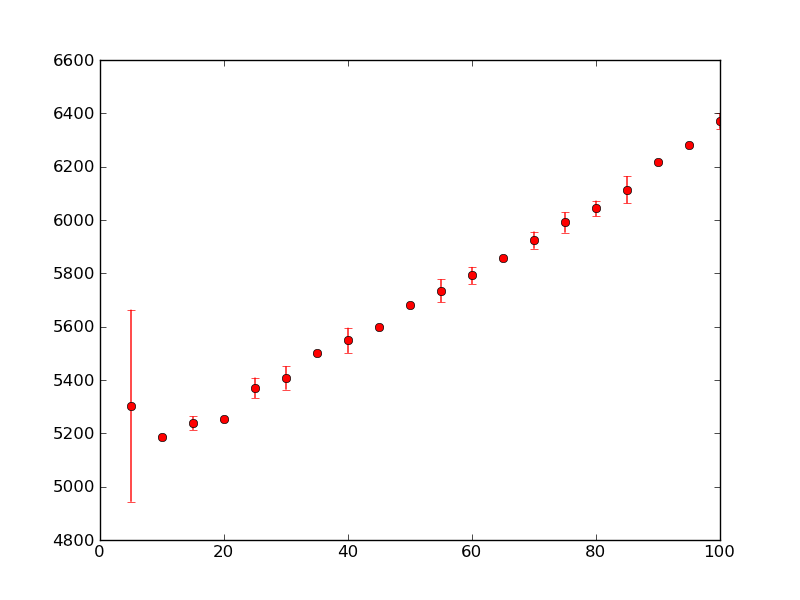
\includegraphics[scale=0.4]{../graphs/categorical/categorical-reduced-c-space.png}
%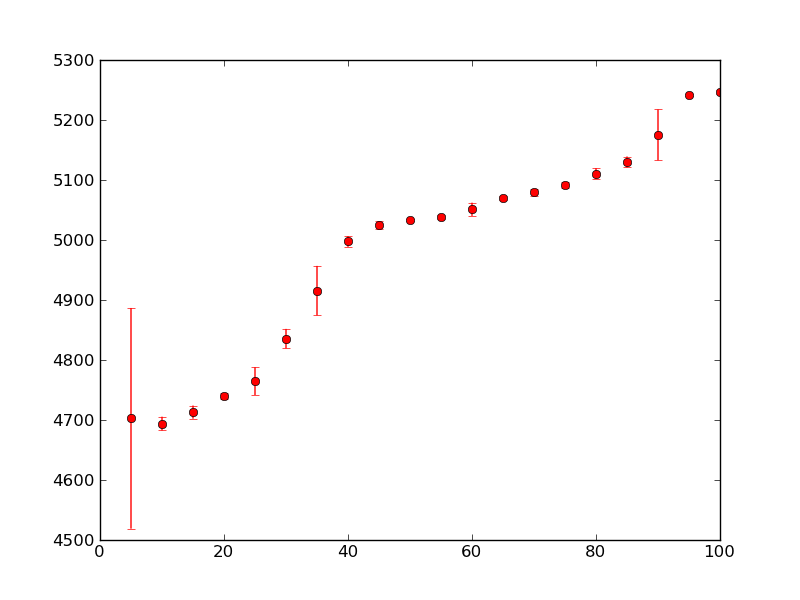
\includegraphics[scale=0.4]{../graphs/categorical/categorical-reduced-py-space.png} \\
%Reduced traces C \qquad \qquad \qquad\qquad\qquad\qquad \qquad Reduced traces Python \\
%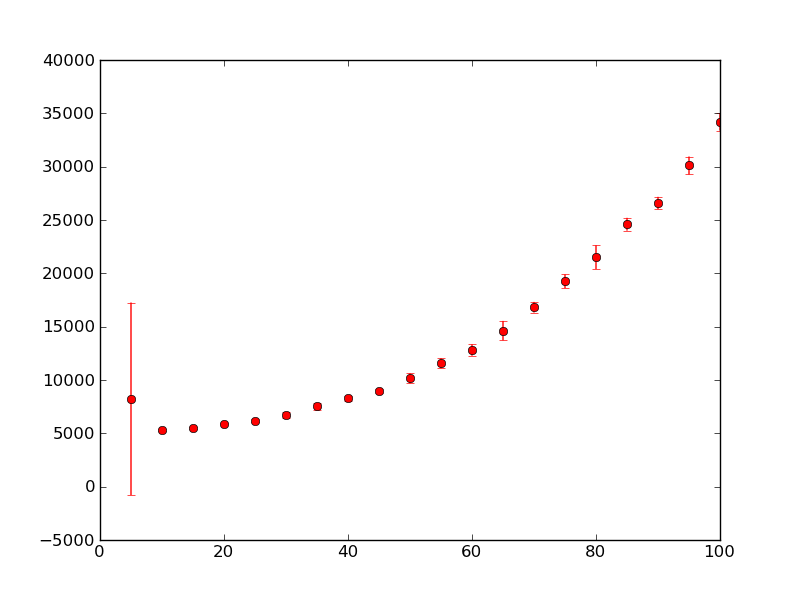
\includegraphics[scale=0.4]{../graphs/categorical/categorical-traces-c-space.png}
%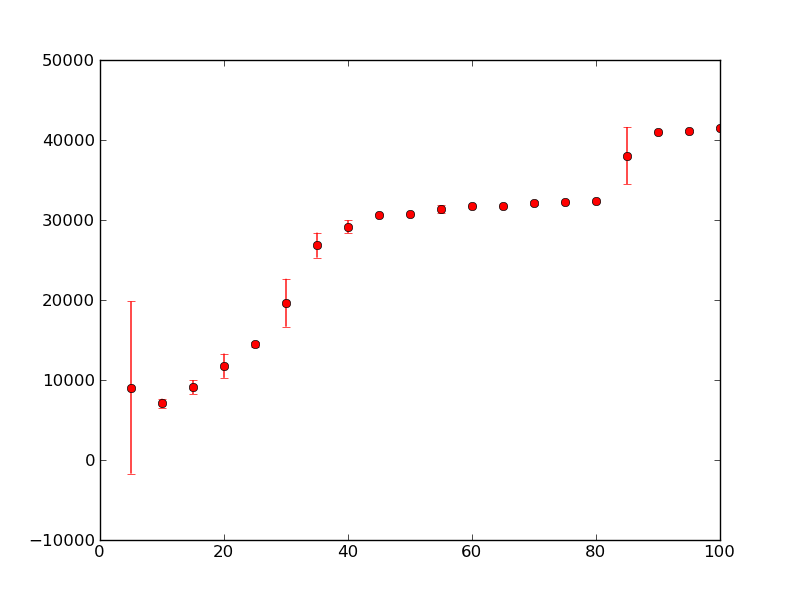
\includegraphics[scale=0.4]{../graphs/categorical/categorical-traces-py-space.png} \\
%Traces C \qquad\qquad\qquad\qquad\qquad\qquad \qquad Traces Python \\
%\pagebreak
%{\bf TIME} \\
%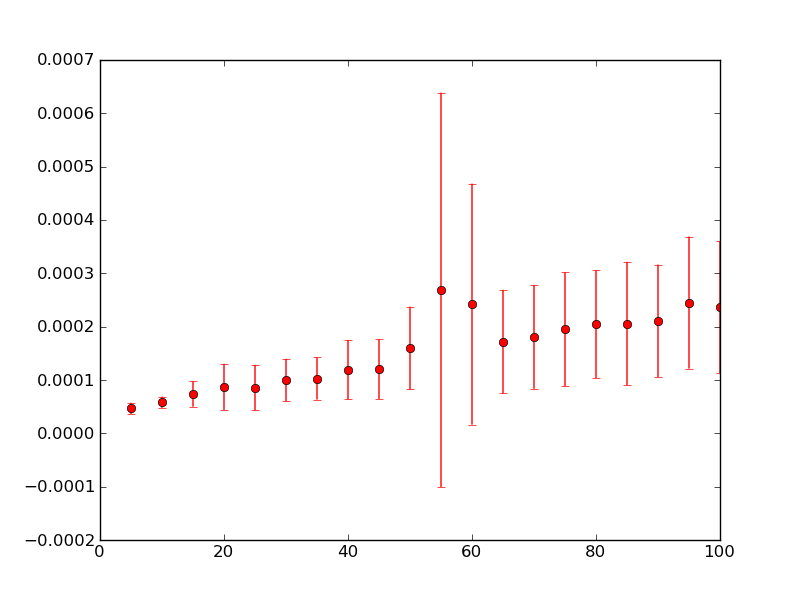
\includegraphics[scale=0.4]{../graphs/categorical/categorical-reduced-c-time.png} 
%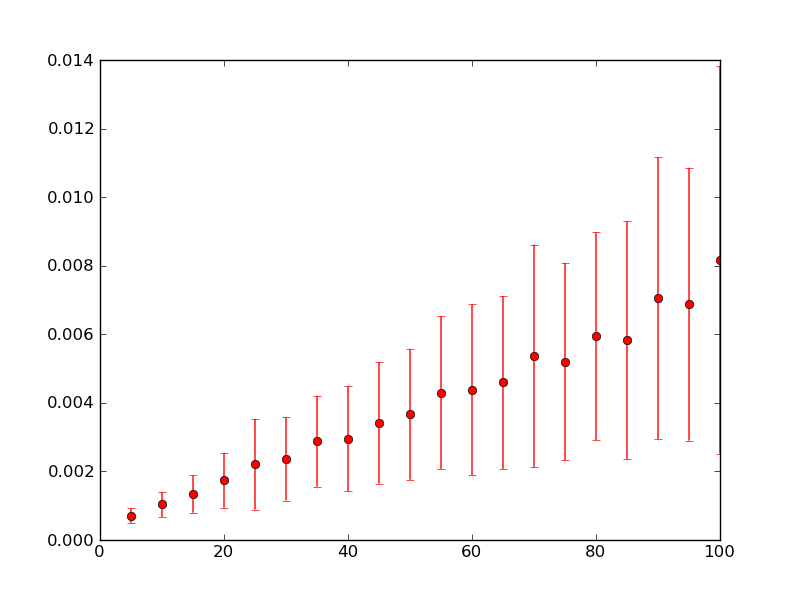
\includegraphics[scale=0.4]{../graphs/categorical/categorical-reduced-py-time.png} \\
%Reduced traces C \qquad \qquad \qquad\qquad\qquad\qquad \qquad Reduced traces Python \\
%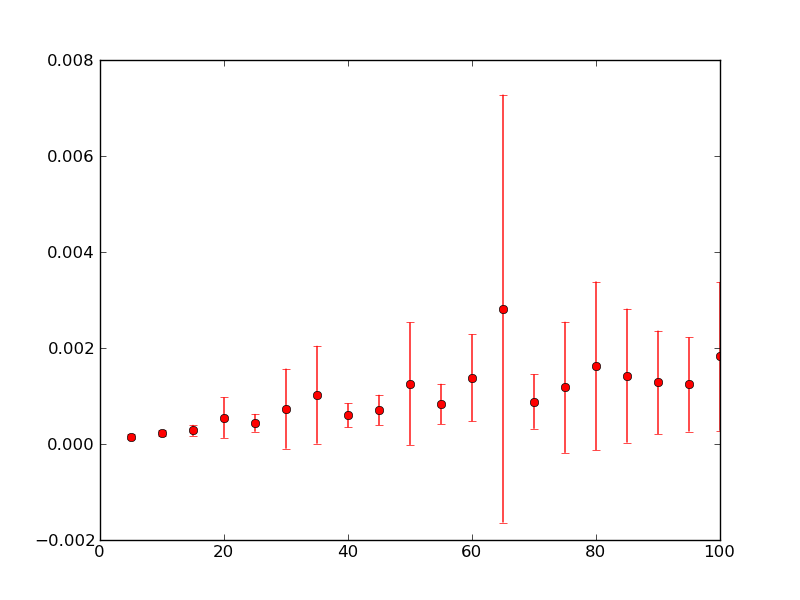
\includegraphics[scale=0.4]{../graphs/categorical/categorical-traces-c-time.png}
%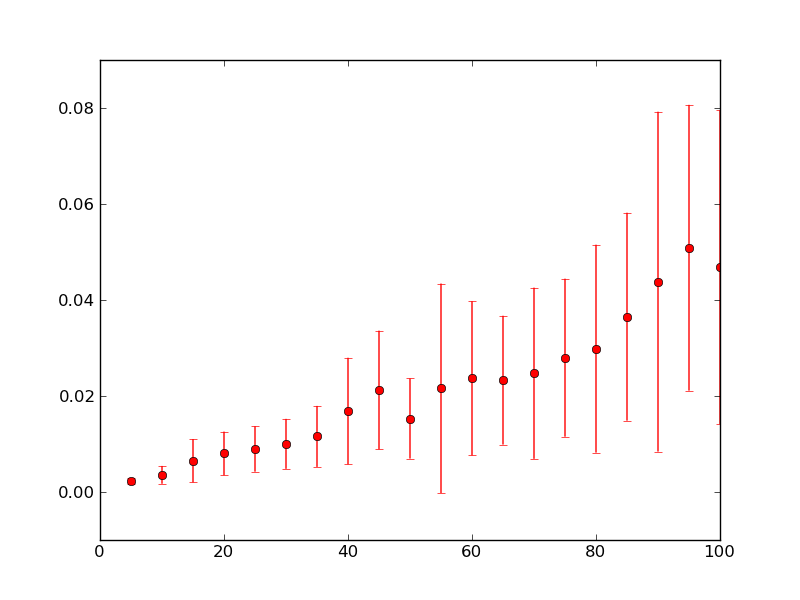
\includegraphics[scale=0.4]{../graphs/categorical/categorical-traces-py-time.png} \\
%Traces C \qquad\qquad\qquad\qquad\qquad\qquad \qquad Traces Python \\
%\end{center}
%%
%%\subsection{A Simple HMM}
%%
%%Suppose we have some integers {\tt nstates}, and {\tt chainlength}.
%%
%%\begin{leftbar} \begin{small} \begin{verbatim}
%%ASSUME get-column (mem (lambda (i) (symmetric-dirichlet 1 nstates)))
%%
%%ASSUME get-next-state 
%%                        (lambda (i) \
%%                                (let ((loop (lambda (v j) \
%%                                      (let ( (w ((get-column i) j))) \
%%                                             (if (< v w) j (loop (- v w) (inc j))))))) \
%%                                (loop (rand) 0)))
%%
%%  ripl.assume("state", lisp_parser.parse("(mem (lambda (i) (if (= i 0) 0 (get-next-state (state (dec i))))))"))
%%
%%  ripl.assume("laststate", lisp_parser.parse("(state chainlength)"))
%%\end{verbatim} \end{small} \end{leftbar}
%%
%%hmm-simple-reduced-traces-py-memory.png
%%hmm-simple-reduced-traces-py-time.png
%%hmm-simple-traces-py-memory.png
%%hmm-simple-traces-py-time.png
%
%\subsection{Topic Modeling}
%
%Consider the following program:
%
%%\begin{leftbar} \begin{small} \begin{verbatim}
%%ASSUME sample-dirichlet (lambda (prob_array) (let ((loop
%%                               (lambda (v i)
%%                                       (let ((w (prob_array i))) 
%%                                            (if (< v w) i (loop (- v w) (+ i 1))))))) 
%%                              (loop (rand) 0)))
%%
%%ASSUME get-document-topic-weights (mem (lambda (doc) (symmetric-dirichlet 1 ntopics)))
%%ASSUME get-document-topic-sampler (mem (lambda (doc) (sample-dirichlet (get-document-topic-weights doc))))
%%ASSUME get-topic-word-weights (mem (lambda (topic) (symmetric-dirichlet 1 nwords)))
%%ASSUME get-topic-word-sampler (mem (lambda (topic) (sample-dirichlet (get-topic-word-weights topic))))
%%
%%
%% ASSUME doc0_word0 (get-topic-word-sampler (get-document-topic-sampler 0))
%%\end{verbatim} \end{small} \end{leftbar}
%
%\begin{leftbar} \begin{small} \begin{verbatim}
%ASSUME get-topic-word-hyper (mem (lambda (topic) (gamma 1 1)))
%ASSUME get-document-topic-hyper (mem (lambda (doc) (gamma 1 1)))
%ASSUME get-document-topic-sampler (mem (lambda (doc) 
%          (symmetric-dirichlet-multinomial/make (/ (get-document-topic-hyper doc) ntopics) ntopics)))
%
%ASSUME get-topic-word-sampler (mem (lambda (topic) 
%          (symmetric-dirichlet-multinomial/make (/ (get-topic-word-hyper topic) nwords) nwords)))
%
%ASSUME get-word (mem (lambda (doc pos) ((get-topic-word-sampler ((get-document-topic-sampler doc))))))
%\end{verbatim} \end{small} \end{leftbar}
%
%When running this program (with increasingly large documents), we see that the space usage is about 50\% better for reduced traces, and the time is about 50\% worse.
%\pagebreak
%\begin{center}
%{\bf SPACE} \\
%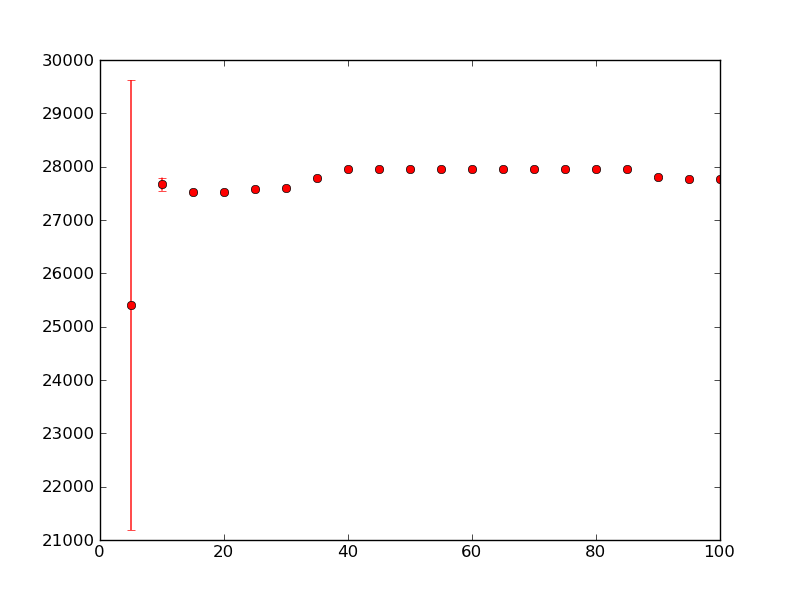
\includegraphics[scale=0.4]{../graphs/topic_models/topic-model-collapsed-traces-py-memory.png} 
%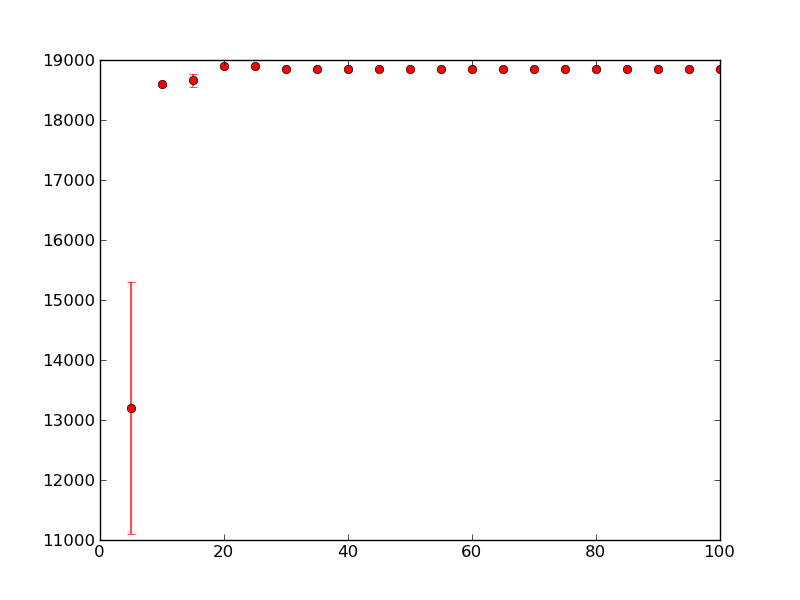
\includegraphics[scale=0.4]{../graphs/topic_models/topic-model-collapsed-reduced-traces-py-memory.png} \\
%Traces Python \qquad \qquad \qquad\qquad\qquad\qquad \qquad Reduced traces Python \\
%{\bf TIME} \\
%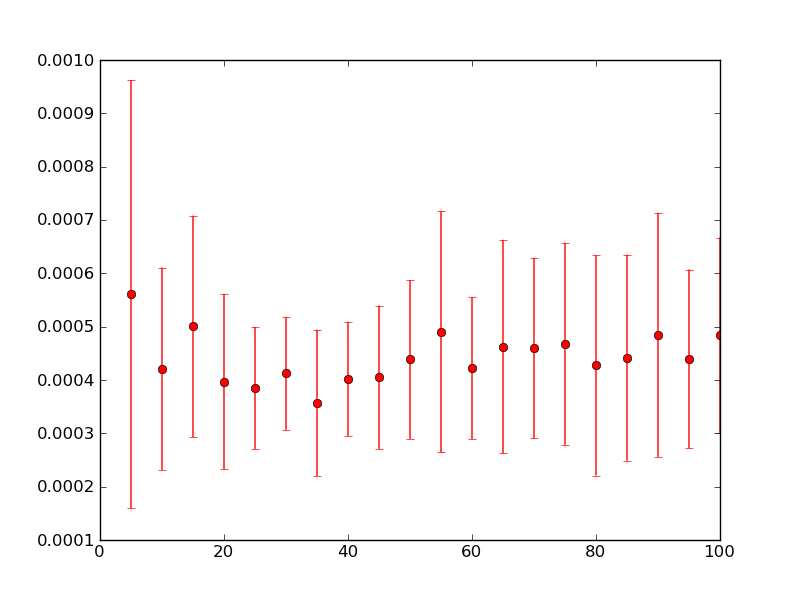
\includegraphics[scale=0.4]{../graphs/topic_models/topic-model-collapsed-traces-py-time.png} 
%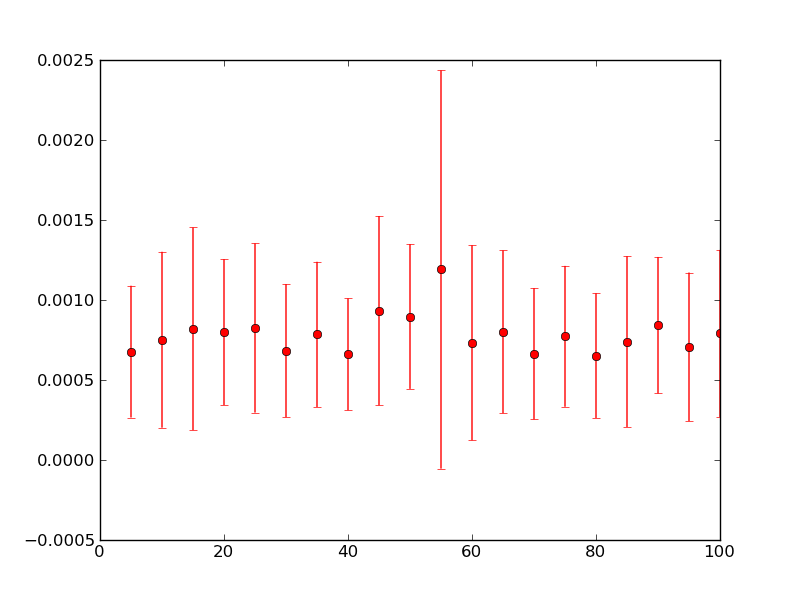
\includegraphics[scale=0.4]{../graphs/topic_models/topic-model-collapsed-reduced-traces-py-time.png} \\
%Traces Python \qquad \qquad \qquad\qquad\qquad\qquad \qquad Reduced traces Python \\
%\end{center}
%In fact, this topic modeling code was used to infer topics from a real corpus of 1500 documents with over a million total words.  The results were quite promising.  The C engine was able to perform on the order of 100,000 inference steps per second, using around 15 gigabytes of RAM.  Here is a graph of the logscore over time:
%
%\begin{center}
%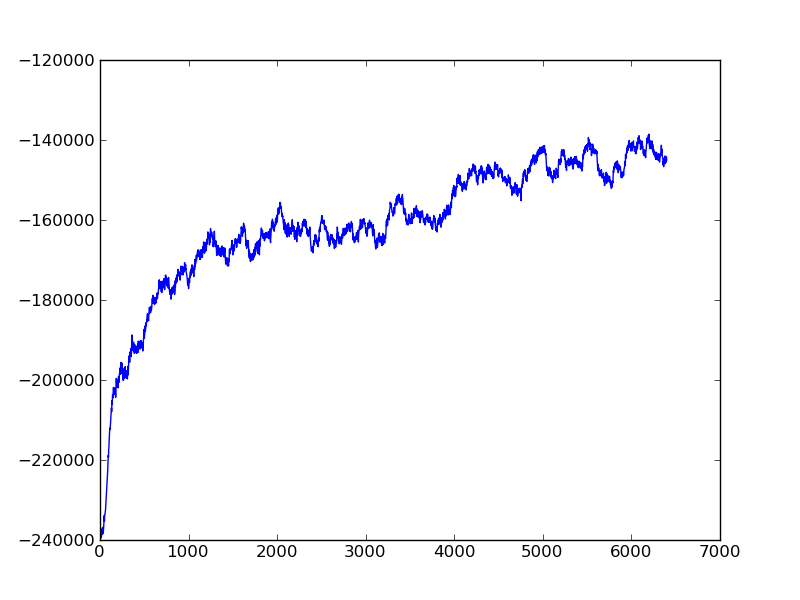
\includegraphics[scale=0.35]{logscores.png} 
%\end{center}
%
%And here is a list of the final topics discovered:
%\begin{verbatim}
%topic 0: model(0.0337) structure(0.0278) algorithm(0.0272) network(0.0259) system(0.0226) sonn(0.0223) number(0.0213) node(0.0209) parameter(0.0181) function(0.0175) neural(0.0163) mdl(0.016) estimation(0.0154) organizing(0.0139) criterion(0.013) performance(0.0125) search(0.0125) input(0.0103) output(0.0101) sec(0.0097)
%topic 1: case(0.0099) fraction(0.0083) training(0.0082) probability(0.0073) weight(0.0069) appreciated(0.0064) compensating(0.0057) sional(0.0006) predictive(0.0005) comparative(0.0005) inferred(0.0005) push(0.0005) schmidt(0.0005) neighbout(0.0005) thn(0.0005) aminergic(0.0005) combiner(0.0005) allinson(0.0005) songbird(0.0005) mrtd(0.0005)
%topic 2: tension(0.0006) lhe(0.0006) extremely(0.0005) inductive(0.0005) modularity(0.0005) ensuring(0.0005) continu(0.0005) kosowsky(0.0005) loth(0.0005) leverages(0.0005) bmu(0.0005) oid(0.0005) ventional(0.0005) creatures(0.0005) approximation(0.0004) simulation(0.0004) provide(0.0004) trajectory(0.0004) world(0.0004) nature(0.0004)
%topic 3: florida(0.0006) frames(0.0005) prototypes(0.0005) genes(0.0005) atr(0.0005) sym(0.0005) benign(0.0005) internally(0.0005) kronecker(0.0005) lstm(0.0005) illill(0.0005) foun(0.0005) tme(0.0005) leary(0.0005) addemup(0.0005) activation(0.0004) statistical(0.0004) synapses(0.0004) validation(0.0004) limited(0.0004)
%topic 4: annealing(0.0262) equilibrium(0.0178) average(0.0175) spin(0.0157) simulated(0.0143) network(0.0134) mean(0.0134) hopfield(0.0109) found(0.0107) operation(0.0107) temperature(0.0107) providing(0.0107) performance(0.0101) nonlinear(0.0081) bin(0.0079) graph(0.0075) case(0.0074) variance(0.0071) system(0.0066) ability(0.0065)
%topic 5: count(0.0088) modify(0.0088) error(0.0082) output(0.008) total(0.0078) numeral(0.0072) set(0.0069) threshold(0.0065) wij(0.005) providence(0.0006) top(0.0005) pole(0.0005) jitter(0.0005) pay(0.0005) neck(0.0005) converting(0.0005) glove(0.0005) analogical(0.0005) symptom(0.0005) extinction(0.0005)
%topic 6: network(0.0412) solution(0.0402) human(0.0379) pattern(0.0339) generalization(0.0317) subject(0.0311) number(0.0246) unit(0.0206) minimal(0.0189) analysis(0.0179) response(0.0161) categorization(0.0151) adaptive(0.015) hidden(0.0141) training(0.0135) initial(0.0126) result(0.0123) problem(0.0121) learning(0.0108) set(0.0102)
%topic 7: solution(0.0221) generalization(0.0174) human(0.0119) cursor(0.0115) network(0.0105) external(0.0077) xor(0.0074) experiment(0.007) response(0.0067) system(0.0066) expected(0.0065) profiles(0.0065) perfusion(0.0065) examine(0.0062) implying(0.0062) inv(0.0062) probabilistic(0.0061) graph(0.006) desired(0.006) artificial(0.0059)
%topic 8: learning(0.0264) point(0.0231) algorithm(0.0195) network(0.0175) function(0.0166) layer(0.0153) local(0.0144) linear(0.0143) error(0.0127) data(0.0122) matrix(0.0118) multi(0.0117) convex(0.0116) set(0.0111) input(0.0104) saddle(0.0103) unit(0.0102) resolution(0.0101) problem(0.0099) real(0.0091)
%topic 9: classifier(0.0933) network(0.0557) system(0.0425) message(0.0407) set(0.0403) match(0.0365) node(0.0343) link(0.028) post(0.0221) neural(0.0204) strength(0.0198) environment(0.019) weight(0.0181) learning(0.0159) algorithm(0.0146) messages(0.0134) nodes(0.0127) bid(0.0121) environmental(0.0118) genetic(0.0117)
%topic 10: dimensional(0.0191) ability(0.0172) sum(0.0108) space(0.0107) input(0.0095) inventory(0.0093) fixed(0.0067) concentric(0.0067) facto(0.0065) eigenvector(0.0064) detail(0.0063) hierarchy(0.0063) lattice(0.0062) integrating(0.0062) associates(0.0062) network(0.0061) level(0.0061) mapping(0.0061) resolution(0.0061) matrices(0.0061)
%topic 11: number(0.0088) conceptual(0.0006) overcomes(0.0006) perceptron(0.0005) development(0.0005) diagonal(0.0005) numerical(0.0005) arithmetic(0.0005) infinitely(0.0005) optima(0.0005) ues(0.0005) laminar(0.0005) triad(0.0005) nism(0.0005) eigenfeatures(0.0005) dynamic(0.0004) measured(0.0004) processes(0.0004) text(0.0004) primary(0.0004)
%topic 12: remarkably(0.0006) doubly(0.0006) herbster(0.0006) net(0.0005) conclusion(0.0005) empirical(0.0005) sides(0.0005) cation(0.0005) tanaka(0.0005) volt(0.0005) dopamine(0.0005) ito(0.0005) weaken(0.0005) lades(0.0005) synchronizing(0.0005) fedorov(0.0005) section(0.0004) computation(0.0004) note(0.0004) modeling(0.0004)
%topic 13: phonetic(0.0007) stationary(0.0006) xij(0.0006) hungry(0.0006) session(0.0005) entered(0.0005) stant(0.0005) symmetrically(0.0005) dam(0.0005) services(0.0005) deterministically(0.0005) eaton(0.0005) dumais(0.0005) siggraph(0.0005) stringent(0.0005) shortening(0.0005) small(0.0004) context(0.0004) chosen(0.0004) evaluation(0.0004)
%topic 14: examples(0.0351) function(0.0333) net(0.0268) threshold(0.0201) nodes(0.0196) random(0.0195) weight(0.0192) bound(0.0182) distribution(0.0168) theorem(0.0166) learning(0.0163) input(0.0156) network(0.0143) node(0.013) layer(0.0128) set(0.0119) size(0.0116) fraction(0.0115) number(0.011) algorithm(0.0109)
%topic 15: lipschitz(0.0081) jaakkola(0.0006) sual(0.0006) synaptic(0.0005) energy(0.0005) combination(0.0005) column(0.0005) technologies(0.0005) factorized(0.0005) decided(0.0005) goldberg(0.0005) ballistic(0.0005) shh(0.0005) hildreth(0.0005) ospf(0.0005) carlson(0.0005) carnevale(0.0005) speech(0.0004) due(0.0004) human(0.0004)
%topic 16: effort(0.0085) britten(0.0085) hopfield(0.0072) rissanen(0.0071) drives(0.0006) accepted(0.0005) designing(0.0005) luminance(0.0005) inhibited(0.0005) strongest(0.0005) leak(0.0005) schematically(0.0005) minimisation(0.0005) overload(0.0005) jmi(0.0005) tsividis(0.0005) collapses(0.0005) cylindrical(0.0005) unify(0.0005) suppose(0.0004)
%topic 17: occlusion(0.0008) wechsler(0.0007) quadratic(0.0006) calcium(0.0006) getting(0.0006) brownlow(0.0006) lwpca(0.0006) requires(0.0005) unlike(0.0005) lack(0.0005) eng(0.0005) isotropic(0.0005) institut(0.0005) inadequate(0.0005) inte(0.0005) sperduti(0.0005) envi(0.0005) sprite(0.0005) ccr(0.0005) diophantine(0.0005)
%topic 18: leading(0.0087) sort(0.0079) gij(0.0006) closure(0.0006) vision(0.0005) inhibition(0.0005) nip(0.0005) nervous(0.0005) handbook(0.0005) inferences(0.0005) invoking(0.0005) trec(0.0005) quiet(0.0005) vos(0.0005) obscure(0.0005) permissible(0.0005) large(0.0004) respect(0.0004) feedback(0.0004) conclusion(0.0004)
%topic 19: resolution(0.028) data(0.025) level(0.0227) hierarchy(0.0198) input(0.0192) function(0.0183) system(0.0169) exemplar(0.0169) multi(0.0155) algorithm(0.014) mapping(0.0138) point(0.0134) problem(0.0131) timeseries(0.0126) training(0.0122) learning(0.0103) adaptive(0.0103) real(0.0102) lookup(0.0092) linear(0.0091)
%topic 20: output(0.0093) bound(0.0087) criterion(0.0066) exhaustively(0.0007) table(0.0006) eoo(0.0006) hold(0.0005) storage(0.0005) workspace(0.0005) reverse(0.0005) severely(0.0005) angeles(0.0005) unrealistic(0.0005) unlearnable(0.0005) matrix(0.0004) computer(0.0004) low(0.0004) markov(0.0004) resulting(0.0004) advances(0.0004)
%topic 21: network(0.0437) output(0.0303) input(0.0259) unit(0.0246) error(0.0223) learning(0.02) algorithm(0.0198) joint(0.0162) layer(0.015) goal(0.0147) problem(0.0144) linear(0.0132) weight(0.0102) hidden(0.0099) arm(0.0095) set(0.0094) vector(0.0089) robot(0.0088) sanger(0.0088) training(0.0086)
%topic 22: cem(0.0006) lung(0.0006) principles(0.0005) concatenated(0.0005) alexander(0.0005) joseph(0.0005) tolerant(0.0005) parcor(0.0005) presidential(0.0005) intend(0.0005) fell(0.0005) tomaso(0.0005) lpc(0.0005) inh(0.0005) malvern(0.0005) reestimate(0.0005) distinctly(0.0005) loglog(0.0005) operation(0.0004) finding(0.0004)
%topic 23: symmetric(0.0005) wind(0.0005) token(0.0005) shepard(0.0005) molecules(0.0005) server(0.0005) differentiate(0.0005) triple(0.0005) blank(0.0005) vaadia(0.0005) reiterant(0.0005) sussex(0.0005) rsp(0.0005) cca(0.0005) dennis(0.0005) graceful(0.0005) tonotopic(0.0005) expert(0.0004) evaluation(0.0004) period(0.0004)
%topic 24: activates(0.0006) obeying(0.0006) refer(0.0005) generic(0.0005) generality(0.0005) minus(0.0005) concentrated(0.0005) copies(0.0005) carries(0.0005) grbf(0.0005) clockwise(0.0005) gmdh(0.0005) emulator(0.0005) identifiable(0.0005) turbo(0.0005) logo(0.0005) kabsch(0.0005) otolith(0.0005) strawman(0.0005) pothesis(0.0005)
%topic 25: sequentially(0.0008) tive(0.0006) timothy(0.0006) kung(0.0006) interna(0.0006) amir(0.0006) fll(0.0006) mension(0.0006) ventional(0.0006) thirteen(0.0006) robust(0.0005) conducted(0.0005) utterances(0.0005) skill(0.0005) token(0.0005) yang(0.0005) helmholtz(0.0005) dmm(0.0005) chi(0.0005) tectum(0.0005)
%topic 26: net(0.0308) examples(0.0279) network(0.0251) function(0.0179) training(0.0177) feedforward(0.0174) learning(0.0166) random(0.0159) nodes(0.0146) corollary(0.0143) linear(0.0137) architecture(0.0133) bound(0.0131) distribution(0.012) future(0.012) layer(0.0116) weight(0.0115) threshold(0.0114) dichotomies(0.0103) algorithm(0.0097)
%topic 27: order(0.0078) search(0.0006) extract(0.0006) ject(0.0006) unix(0.0005) cocktail(0.0005) hin(0.0005) olution(0.0005) diate(0.0005) level(0.0004) negative(0.0004) equivalent(0.0004) design(0.0004) york(0.0004) similarity(0.0004) hebbian(0.0004) numerical(0.0004) presentation(0.0004) closely(0.0004) composed(0.0004)
%topic 28: initializes(0.0006) tuning(0.0005) structural(0.0005) ideas(0.0005) geiger(0.0005) opponent(0.0005) perturbing(0.0005) pnas(0.0005) decomposes(0.0005) diabetes(0.0005) eoo(0.0005) eec(0.0005) decent(0.0005) smeared(0.0005) alphas(0.0005) kent(0.0005) computer(0.0004) study(0.0004) processes(0.0004) face(0.0004)
%topic 29: restrictive(0.0006) broadcast(0.0006) implicated(0.0006) patch(0.0005) replica(0.0005) slice(0.0005) ron(0.0005) hme(0.0005) big(0.0005) amherst(0.0005) latency(0.0005) ben(0.0005) triple(0.0005) dead(0.0005) rec(0.0005) pushdown(0.0005) sory(0.0005) sullivan(0.0005) neurogenesy(0.0005) mesterharm(0.0005)
%topic 30: output(0.0256) wij(0.0157) hidden(0.0152) number(0.0116) current(0.0114) weight(0.0107) unit(0.0106) problem(0.0105) table(0.0101) integer(0.0084) input(0.0078) pattern(0.0067) presented(0.0067) median(0.0067) representation(0.0065) plr(0.0064) learning(0.0062) view(0.0061) perceptton(0.0061) architecture(0.006)
%topic 31: occipital(0.0006) set(0.0005) neuron(0.0005) curve(0.0005) crossing(0.0005) incoming(0.0005) washington(0.0005) intrator(0.0005) obermayer(0.0005) cylinder(0.0005) attributed(0.0005) imaginary(0.0005) saturates(0.0005) gary(0.0005) refining(0.0005) isolate(0.0005) genevieve(0.0005) spectively(0.0005) holler(0.0005) bayesian(0.0004)
%topic 32: extensively(0.0006) gpp(0.0006) curve(0.0005) mlp(0.0005) nucleus(0.0005) autonomous(0.0005) paul(0.0005) echoes(0.0005) crosses(0.0005) preferences(0.0005) auxiliary(0.0005) formulae(0.0005) strongest(0.0005) quadrature(0.0005) dig(0.0005) deemed(0.0005) vedelsby(0.0005) til(0.0005) ickinger(0.0005) thirdly(0.0005)
%topic 33: mfa(0.0241) mean(0.0238) field(0.019) annealing(0.0143) averages(0.0127) problem(0.0103) operation(0.0101) network(0.0097) algorithm(0.0096) graph(0.0096) force(0.0094) hopfield(0.0093) simulated(0.0086) temperature(0.0086) compared(0.0084) speedup(0.0081) ece(0.0067) cease(0.0064) optimum(0.0061) analytically(0.006)
%topic 34: sphering(0.0059) marginally(0.0007) ebl(0.0006) aspect(0.0005) published(0.0005) file(0.0005) contrary(0.0005) rapture(0.0005) albeit(0.0005) stochas(0.0005) gsm(0.0005) ade(0.0005) posture(0.0005) hummel(0.0005) misadjustment(0.0005) troublesome(0.0005) progressive(0.0005) current(0.0004) press(0.0004) domain(0.0004)
%topic 35: hidden(0.0085) perform(0.0084) internal(0.0084) algorithm(0.0081) exact(0.0078) solve(0.0078) process(0.0076) learning(0.0072) pattern(0.0069) plr(0.0065) row(0.0063) fail(0.0063) sharpness(0.006) output(0.0057) training(0.0056) nadel(0.0006) prc(0.0006) provided(0.0005) presence(0.0005) mem(0.0005)
%topic 36: learning(0.0257) function(0.0161) resolution(0.0154) input(0.0152) lattice(0.0148) system(0.0143) representation(0.0139) table(0.0137) problem(0.0136) point(0.0135) training(0.0134) data(0.0127) weight(0.0125) output(0.0124) network(0.0123) algorithm(0.0123) set(0.012) internal(0.0118) space(0.0109) error(0.0103)
%topic 37: network(0.0644) subject(0.0351) solution(0.0289) human(0.028) pattern(0.0174) minimal(0.0174) learning(0.0169) analysis(0.0165) hidden(0.0157) training(0.0149) adaptive(0.0143) initial(0.0137) unit(0.0128) profiles(0.0123) generalization(0.0114) find(0.0108) dimension(0.0103) problem(0.0099) finding(0.0091) profile(0.009)
%topic 38: learning(0.0326) internal(0.0302) input(0.0271) representation(0.0267) layer(0.0237) algorithm(0.0225) network(0.0208) unit(0.0207) output(0.0205) plr(0.0197) weight(0.019) hidden(0.0186) number(0.0176) table(0.016) solution(0.0154) training(0.0146) pattern(0.0128) set(0.0126) problem(0.0121) values(0.0112)
%topic 39: learning(0.0419) problem(0.0393) algorithm(0.0374) vector(0.0221) propagation(0.0202) function(0.0195) gradient(0.0186) network(0.0183) weight(0.0157) descent(0.0153) steepest(0.0153) optimization(0.0152) error(0.0147) convergence(0.0139) set(0.0135) input(0.0131) method(0.0124) techniques(0.0122) unit(0.0121) parallel(0.0119)
%topic 40: pasadena(0.0087) unit(0.008) data(0.0079) truncating(0.0079) model(0.0078) output(0.007) lattice(0.007) space(0.0006) comparable(0.0006) roc(0.0006) corr(0.0006) finland(0.0006) finite(0.0005) server(0.0005) inserted(0.0005) crf(0.0005) mae(0.0005) numeric(0.0005) arx(0.0005) balltree(0.0005)
%topic 41: appealing(0.014) function(0.0139) problem(0.0131) generate(0.0083) paper(0.008) set(0.0078) equation(0.0076) factored(0.0076) farmer(0.0074) lattice(0.0073) processing(0.0071) propagation(0.007) performance(0.0069) obtainable(0.0067) data(0.0065) prediction(0.0065) table(0.0065) values(0.0063) computation(0.006) spline(0.006)
%topic 42: mean(0.0363) field(0.0331) mfa(0.0327) spin(0.0317) temperature(0.0256) graph(0.0234) problem(0.0181) average(0.0178) solution(0.0158) averages(0.0156) annealing(0.0155) ssa(0.0147) simulated(0.0143) network(0.0142) iteration(0.0133) nodes(0.013) system(0.0129) point(0.0117) optimization(0.0113) hopfield(0.0111)
%topic 43: levy(0.0006) rosci(0.0006) excised(0.0006) identical(0.0005) carried(0.0005) composition(0.0005) writer(0.0005) hrr(0.0005) smear(0.0005) passage(0.0005) rolling(0.0005) steep(0.0005) rvm(0.0005) arose(0.0005) mhaskar(0.0005) chernoff(0.0005) impression(0.0005) seeger(0.0005) analysis(0.0004) rule(0.0004)
%topic 44: increased(0.0005) multilayer(0.0005) beginning(0.0005) saturation(0.0005) unlikely(0.0005) funded(0.0005) shawe(0.0005) oam(0.0005) stochasticity(0.0005) nen(0.0005) engr(0.0005) escapes(0.0005) conceived(0.0005) method(0.0004) seen(0.0004) common(0.0004) magnitude(0.0004) estimating(0.0004) connectivity(0.0004) partially(0.0004)
%topic 45: unit(0.0087) choice(0.0087) hidden(0.0081) problem(0.0074) row(0.0072) parity(0.0058) discard(0.0006) suppresses(0.0006) accumulated(0.0005) syllables(0.0005) interspike(0.0005) functionally(0.0005) accessible(0.0005) hexagonal(0.0005) asynchronously(0.0005) deviates(0.0005) orthographic(0.0005) wsj(0.0005) schyn(0.0005) current(0.0004)
%topic 46: slot(0.0007) traffic(0.0006) critical(0.0005) bandwidth(0.0005) trace(0.0005) jacobian(0.0005) alternatively(0.0005) andreou(0.0005) tar(0.0005) analogously(0.0005) cov(0.0005) barrett(0.0005) shear(0.0005) ule(0.0005) riesenhuber(0.0005) nnl(0.0005) parallelizable(0.0005) elf(0.0005) lftc(0.0005) chl(0.0005)
%topic 47: distributed(0.0005) clearly(0.0005) hardware(0.0005) subspace(0.0005) begin(0.0005) improving(0.0005) straight(0.0005) continuously(0.0005) psychophysical(0.0005) nonetheless(0.0005) heavily(0.0005) graf(0.0005) nih(0.0005) scientist(0.0005) shi(0.0005) symmetries(0.0005) oooo(0.0005) embodies(0.0005) amap(0.0005) echolocation(0.0005)
%topic 48: psth(0.0006) implies(0.0005) spectrum(0.0005) formation(0.0005) splines(0.0005) poorly(0.0005) annealed(0.0005) conjecture(0.0005) optimisation(0.0005) believed(0.0005) hebrew(0.0005) boxlet(0.0005) primed(0.0005) steep(0.0005) donoho(0.0005) mdac(0.0005) trl(0.0005) brunel(0.0005) popularity(0.0005) ssp(0.0005)
%topic 49: network(0.008) uyar(0.0007) think(0.0006) srn(0.0006) coggin(0.0006) oracle(0.0006) garzon(0.0006) capacity(0.0005) actor(0.0005) cognition(0.0005) dealing(0.0005) captures(0.0005) ave(0.0005) named(0.0005) sector(0.0005) cgm(0.0005) zue(0.0005) browsing(0.0005) gabaergic(0.0005) mrsh(0.0005)
%
%\end{verbatim}
%
%\subsection{CRP Mixture Model}
%
%Lastly, we compared the two engines on a CRP mixture model.
%
%\begin{leftbar} \begin{small} \begin{verbatim}
%
%ASSUME alpha (gamma 0.1 20)
%ASSUME cluster-crp (CRP/make alpha)
%
%ASSUME get-cluster-mean (mem (lambda (cluster) (gaussian 0 10)))
%ASSUME get-cluster-variance (mem (lambda (cluster) (gamma 0.1 100)))
%ASSUME get-cluster (mem (lambda (id) (cluster-crp)))
%ASSUME get-cluster-model (mem (lambda (cluster) (lambda ( ) (gaussian (get-cluster-mean cluster) (get-cluster-variance cluster)))))
%ASSUME get-datapoint (mem (lambda (id) (gaussian ((get-cluster-model (get-cluster id))) 0.1)))
%\end{verbatim} \end{small} \end{leftbar}
%
%Again, we see an improvement in space usage, and a hit in runtime.
%
%\begin{center}
%{\bf SPACE} \\
%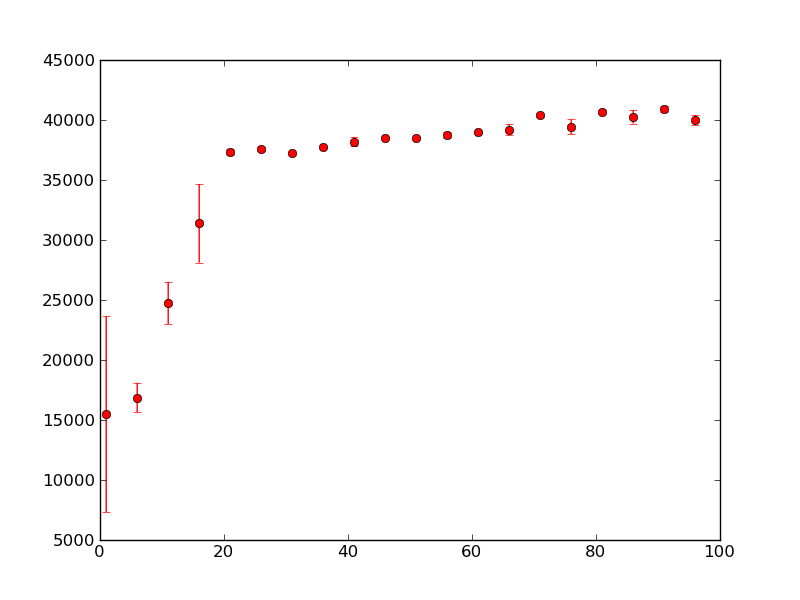
\includegraphics[scale=0.4]{../graphs/CRP_mixture/CRP-mixture-model-collapsed-traces-py-memory.png} 
%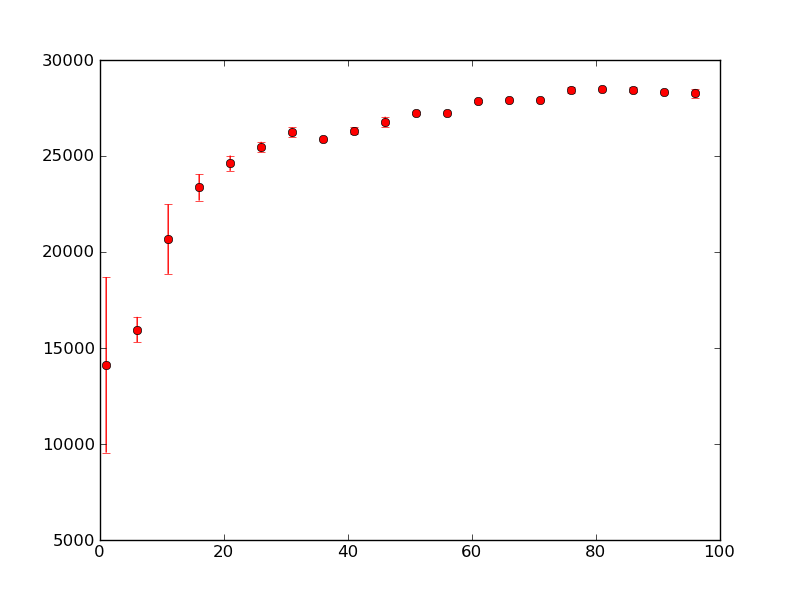
\includegraphics[scale=0.4]{../graphs/CRP_mixture/CRP-mixture-model-collapsed-reduced-traces-py-memory.png} \\
%Traces Python \qquad \qquad \qquad\qquad\qquad\qquad \qquad Reduced traces Python \\
%{\bf TIME} \\
%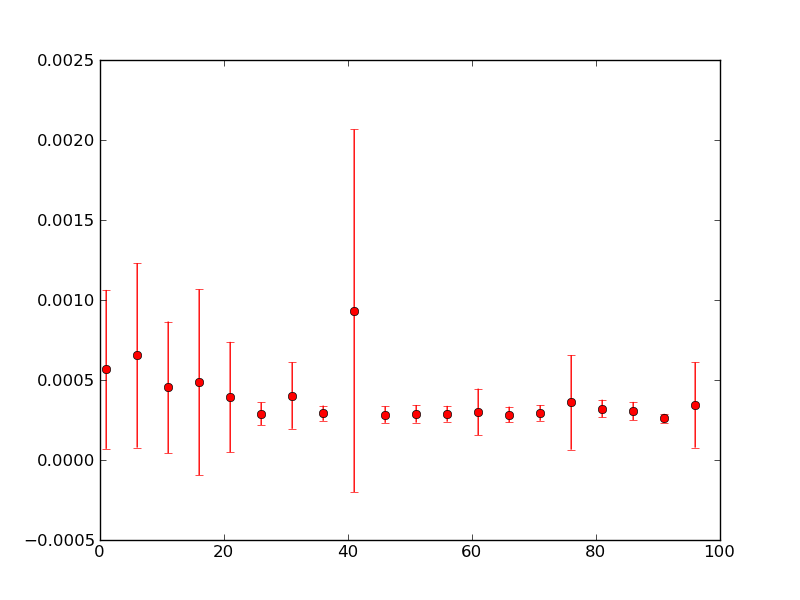
\includegraphics[scale=0.4]{../graphs/CRP_mixture/CRP-mixture-model-collapsed-traces-py-time.png} 
%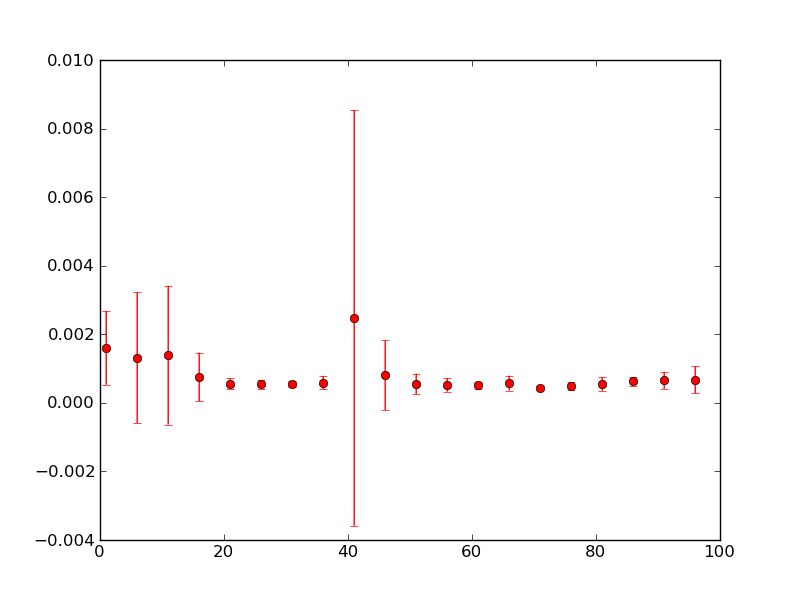
\includegraphics[scale=0.4]{../graphs/CRP_mixture/CRP-mixture-model-collapsed-reduced-traces-py-time.png} \\
%Traces Python \qquad \qquad \qquad\qquad\qquad\qquad \qquad Reduced traces Python \\
%

%\end{center}

\pagebreak
%
%
%\section{Inference}
%In order to perform inference, we must store all random choices (XRP applications) in the execution of our program, so that we can evaluate and unevaluate.  
%
%The first challenge is figuring out how to specify points in the execution history.  Essentially, we use a call stack, augmented with things telling us the location being considered within an expression.  
%
%Then, our database supports the following operations:
%
%\begin{itemize}
%\item {\tt insert(stack, xrp, value, args, obs)}:  Records that the {\tt xrp} applied to {\tt args}, at execution point specified by {\tt stack}, returned {\tt value}.  The argument {\tt obs} specifies whether this was an outermost ``noise" XRP application in an observation.  
%\item {\tt remove(stack)}:  Removes the random choice at the execution point specified by {\tt stack}.  
%\item {\tt has(stack)}:  Checks if the current execution history reaches the execution point specified by {\tt stack}.  
%\item {\tt get(stack)}:  Gets a tuple {\tt (xrp, args, value, prob, obs)} containing all the relevant data corresponding to the random choice stored at {\tt stack}.  The elements of the tuple are, in order:  the XRP applied, the list of arguments, the resulting value, the probability of getting that value, and whether it was an outermost ``noise" application in an observation.
%\item {\tt random\_stack()}:  Return a random stack in the database such that {\tt obs = False}.  
%\item {\tt unevaluate(stack, args)}: Unevaluates everything in the database which was evaluated as a result of reaching the execution point {\tt stack}.  If {\tt args} is provided, then we unevaluate anything evaluated when applying the procedure at {\tt stack} to arguments different from {\tt args}.
%\item {\tt save()}: Saves the current state of the database.
%\item {\tt restore()}: Restores the saved version of the database.
%\item {\tt reset()}: Resets the database, as if the program has not been executed at all.  
%\end{itemize}
%Our database also maintains the following variables:
%\begin{itemize}
%\item {\tt count}:  The number of XRP applications which aren't outermost noise applications.
%\item {\tt prob}:  The product of all probabilities stored, i.e. the probability of the current execution history.
%\item {\tt eval\_prob}:  The product of all probabilities which were newly evaluated since the last save.
%\item {\tt uneval\_prob}:  The product of all probabilities which were unevaluated since the last save.
%\end{itemize}
%
%Implementation of this database is not important.  The main difficulties are in keeping track of location correctly.  %All data is stored in a hash table.  Furthermore, we use an algorithmic trick to augment hash tables to be able to choose a random key in $O(1)$, in order to support {\tt random\_stack()}.  Outermost noise applications are stored separately.   Save does not literally remember the state.  We simply start remembering all inserts and removes, and undo them when we restore.  
%We can now give code for {\tt infer}, which runs a single step in the Markov chain:
%
%\begin{small}
%\begin{verbatim}
%def infer():
%  stack = randomDB.random_stack()
%  (xrp, args, val, prob, obs) = randomDB.get(stack)
%
%  old_p = randomDB.prob
%  old_count = randomDB.count
%
%  randomDB.save()
%
%  randomDB.remove(stack)
%  new_val = xrp.apply(args)
%  randomDB.insert(stack, xrp, new_val, args)
%
%  rerun()
%  
%  new_p = randomDB.prob
%  new_to_old_q = randomDB.uneval_prob / randomDB.count
%  old_to_new_q = randomDB.eval_prob / old_count
%  
%  if new_p * new_to_old_q < old_p * old_to_new_q * random.random():
%    randomDB.restore()
%\end{verbatim}
%\end{small}
%
%
%\noindent Here, {\tt rerun()} simply reruns the entire program, using the new randomness in the DB, evaluating new things and unevaluating neglected things as needed.  It is not hard to verify that this uses the correct probability of transitioning, according to Metropolis-Hastings.  
%
%Technically, we use log probabilities instead of probabilities, as done here, to avoid precision errors.  In fact, we require that the {\tt prob()} function of XRPs return the log probability.
%
%
%% : MH on random worlds
%%            - pseudcode, reflecting what you learned (beyond what was in the AISTATS paper)
%%            - discuss eval, uneval, XRPs with state, mem as an example, etc
%%        - [[whatever focused experiments/results we come up with]]
%
%%\cite{Fagin1}:  
%
%
%
%
%\section{Test Cases}
%
%In order to ensure the language was working properly, a suite of test cases was developed.  
%
%One of the primary techniques used for testing was ``following the prior", using the function {\tt follow\_prior(variable, niters, burnin)}.  To follow the prior, we draw {\tt niters} samples from the prior, and run each of them {\tt burnin} steps in the random walk.  We then view the resulting distribution on {\tt variable}.  % generalize this to view joints on many variables
%
%Here are some of the more illustrative and interesting test cases.
%
%
%\subsection{Testing a tricky coin}
%
%Consider the following scenario:  There is a coin that is fair with probability 50\%.  The rest of the time, its weight is drawn uniformly from the interval [0, 1].  The coin is flipped, and we observe it to be heads {\tt nheads} times.  We then infer the posterior probability that the coin was fair. 
%
%\begin{small}
%\begin{verbatim}
%>>>  noise_level = .001
%>>>  nheads = 1
%>>>  
%>>>  assume('weight', beta(1, 1))
%>>>  assume('tricky-coin', function([], bernoulli('weight')))
%>>>  assume('fair-coin', function([], bernoulli(0.5)))
%>>>  assume('is-fair', bernoulli(0.5))
%>>>  assume('coin', ifelse('is-fair', 'fair-coin', 'tricky-coin')) 
%>>>
%>>>  for i in xrange(nheads):
%>>>    observe(bernoulli_noise(apply('coin'), noise_level), True)
%>>>
%>>>  follow_prior('is-fair', 10000, 1000)
%\end{verbatim}
%\end{small}
%
%% could change to if fair, weight = blah...
%% the way it's coded matters.
%
%We should be able to predict the results of running this program for different values of {\tt nheads}.  First we compute the probability that the coin comes up heads $n$ times, given that it is tricky.  The probability is simply $\beta(1, n + 1) = \frac{1}{n +1}$.  Thus the probability the coin is fair (not tricky), given it came up heads $n$ times, is, by Baye's law $$\frac{\frac{1}{2} \cdot \frac{1}{2^n}}{\frac{1}{2} \cdot \frac{1}{n+1} + \frac{1}{2} \cdot \frac{1}{2^n}} = \frac{n+1}{ 2^n + n+1}.$$
%
%Here are our results, when running {\tt follow\_prior('is-fair', 10000, 1000)}, for the percentage of times the coin was fair:  
%
%\begin{center}
%\begin{tabular}{|c | c| c |} \hline
%{\tt nheads} & Predicted & Actual \\ \hline
%0 & 0.5 & 0.4982\\ \hline
%1 & 0.5 & 0.4934 \\ \hline
%2 & 0.4286 &  0.4289 \\ \hline
%3 & 0.3333 &  0.3346 \\ \hline
%4 & 0.2381 &  0.2712 \\ \hline
%5 & 0.1579 &  0.2528 \\ \hline
%\end{tabular}
%\end{center}
%
%As {\tt nheads} grows, we should expect the mixing time to grow.  This is because 
%\subsection{Bayes nets}
%
%We first test that inference works, by considering a number of test cases.  A classic inference problem which is well understood, is inference in Bayesian networks.  Bayesian networks are incredibly easy to describe in our language.  Here are some simple examples of inference giving the correct answer in a Bayesian network.
%
%\subsubsection{Sprinkler net}
%
%Let's start with a simple example, to get familiar with our language.   Here's a definition of a bayesian network with just two nodes.
%
%\begin{small}
%\begin{verbatim}
%>>> assume('cloudy', bernoulli(0.5))
%>>> assume('sprinkler', ifelse('cloudy', bernoulli(0.1), bernoulli(0.5)))
%\end{verbatim}
%\end{small}
%
%\noindent We then observe that the sprinkler is on.  Worlds in which the sprinkler is on are weighted as 100 times more likely than ones in which the sprinkler is off.  
%
%\begin{small}
%\begin{verbatim}
%>>> noise_level = .01
%>>> sprinkler_ob = observe(bernoulli_noise('sprinkler', noise_level), True)
%\end{verbatim}
%\end{small}
%
%\noindent Now, let's try inferring the weather.  We follow the prior 10000 times, going 50 steps each time.  
%
%\begin{small}
%\begin{verbatim}
%>>> follow_prior('cloudy', 10000, 50)}
%{False: 0.82010000000000005, True: 0.1799}
%\end{verbatim}
%\end{small}
%
%This is close to the value of $\frac{5}{6} = 0.8\overline{333}$ False, which is what we'd get if there was noise in our observation.  However, there is still a number of worlds in which the sprinkler was actually on.  In those worlds, the weather was 50/50.  Thus we should've expect the answer to be on the order of 0.01 lower.  \vspace{6 pt}
%
%Now, let's suppose we didn't observe the sprinkler being on, after all.
%
%% Part of the error is because of the noise.  
%
%\begin{small}
%\begin{verbatim} 
%>>> forget(sprinkler_ob)
%\end{verbatim}
%\end{small}
%
%\noindent So it should be the case that it's cloudy exactly half the time.
%
%\begin{small}
%\begin{verbatim}
%>>> follow_prior('cloudy', 10000, 50)}
%{False: 0.50429999999999997, True: 0.49569999999999997}
%\end{verbatim}
%\end{small}
%
%\noindent  Now, we re-observe the sprinkler to be on.  This time, we are much more sure.
%
%\begin{small}
%\begin{verbatim}
%>>> noise_level = .001
%>>> sprinkler_ob = observe(bernoulli_noise('sprinkler', noise_level), True)
%>>> follow_prior('cloudy', 10000, 50)}
%{False: 0.83999999999999997, True: 0.16}
%\end{verbatim}
%\end{small}
%
%\noindent We see that our answer is even closer to the value of $\frac{5}{6} = 0.8\overline{333}$ False, now.
%
%\subsubsection{Alarm net}
%
%Here's a more complicated Bayesian network, which is given as an example in the classic AI textbook Artificial Intelligence (A Modern Approach).  
%\begin{center} 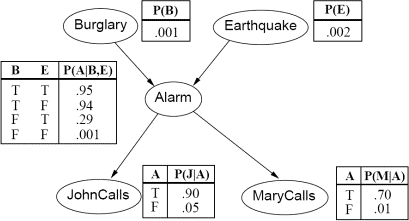
\includegraphics{burglary.png} \end{center}
%
%\noindent Let's define this Bayesian network.
%
%\begin{small}
%\begin{verbatim}
%>>> assume('burglary', bernoulli(0.001))
%>>> assume('earthquake', bernoulli(0.002))
%>>> assume('alarm', ifelse('burglary', ifelse('earthquake', bernoulli(0.95), bernoulli(0.94)), \
%...                                    ifelse('earthquake', bernoulli(0.29), bernoulli(0.001))))
%>>> assume('johnCalls', ifelse('alarm',  bernoulli(0.9), bernoulli(0.05)))
%>>> assume('maryCalls', ifelse('alarm',  bernoulli(0.7), bernoulli(0.01)))
%\end{verbatim}
%\end{small}
%
%\noindent Let's try a couple inference problems.
%
%\begin{small}
%\begin{verbatim}
%>>> follow_prior('alarm', 1000, 100) # should give 0.002516 True
%{False: 0.99739999999999995, True: 0.0025999999999999999}
%>>>
%>>> noise_level = .001
%>>> mary_ob = observe(bernoulli_noise('maryCalls', noise_level), True)
%>>> follow_prior('johnCalls', 1000, 100) # should give 0.177577 True
%{False: 0.91620000000000001, True: 0.083799999999999999}
%>>>
%>>> forget(mary_ob)
%>>> burglary_ob = observe(bernoulli_noise(negation('burglary'), noise_level), True)
%>>> follow_prior('johnCalls', 1000, 100) # should give 0.051343 True
%{False: 0.94710000000000005, True: 0.052900000000000003}
%\end{verbatim}
%\end{small}
%
%The first and third inferences were on the mark, but the second one was off by a factor of two!   The explanation is that Mary calls very rarely calls.  Indeed, she only calls about 0.01 of the time, since the alarm almost never sounds.  This is rare enough that our observation that she called is reasonably likely to be wrong.  In worlds where she doesn't call, John also tends not to call, thus accounting for the large dip. \vspace{6 pt}
%
%To verify that this is the explanation, we can alter the probabilities so that Mary calling is more likely.  Here is an example of this being done.
%
%\begin{small}
%\begin{verbatim}
%>>> reset()
%>>>
%>>> assume('burglary', bernoulli(0.1))
%>>> assume('earthquake', bernoulli(0.2))
%>>> assume('alarm', ifelse('burglary', ifelse('earthquake', bernoulli(0.95), bernoulli(0.94)), \
%...                                    ifelse('earthquake', bernoulli(0.29), bernoulli(0.10))))
%>>> assume('johnCalls', ifelse('alarm',  bernoulli(0.9), bernoulli(0.5)))
%>>> assume('maryCalls', ifelse('alarm',  bernoulli(0.7), bernoulli(0.1)))
%>>>
%>>> follow_prior('alarm', 1000, 100) # should give 0.218400 True
%{False: 0.77959999999999996, True: 0.22040000000000001}
%>>>
%>>> noise_level = .001
%>>> mary_ob = observe(bernoulli_noise('maryCalls', noise_level), True)
%>>> follow_prior('johnCalls', 1000, 100) # should give 0.764681 True
%{False: 0.2432, True: 0.75680000000000003}
%>>>
%>>> forget(mary_ob)
%>>> burglary_ob = observe(bernoulli_noise(negation('burglary'), noise_level), True)
%>>> follow_prior('johnCalls', 1000, 100) # should give 0.561333 True
%{False: 0.44290000000000002, True: 0.55710000000000004}
%\end{verbatim}
%\end{small}
%
%\noindent Success!
%
%
%\subsection{Testing xor}
%
%\noindent Consider the following program, where we simply draw two booleans {\tt a} and {\tt b}, and observe that their xor is {\tt True}:
%
%\begin{small}
%\begin{verbatim}
%>>> p, q = 0.6, 0.4
%>>> noise_level = .01
%>>>
%>>> assume('a', bernoulli(p))
%>>> assume('b', bernoulli(q))
%>>> assume('c', var('a') ^ var('b'))
%>>>
%>>> follow_prior('a', 10000, 100) # should be 0.60 True
%{False: 0.3977, True: 0.60229999999999995}
%>>>
%>>> xor_ob = observe(bernoulli_noise('c', noise_level), True)
%>>> follow_prior('a', 10000, 100) # should be 0.69 True
%{False: 0.3342, True: 0.66579999999999995}
%\end{verbatim}
%\end{small}
%
%
%
%This second inference is significantly off, and it's not the case that our observation is particularly unlikely.  Here, the burn-in was not enough.  Notice that in order to mix, the program must walk over states which contradict the observed values.  
%
%Suppose we are in the state {\tt \{a:True, b:True\}}.  Then, the random walk is highly discouraged from entering either of the two adjacent states {\tt \{a:True, b:False\}} and {\tt \{a:False, b:True\}}, since worlds in which {\tt a$\oplus$b} is {\tt False} are weighted against, by a factor of 100.  
%
%Let's estimate the amount of burn-in it should take for this random walk to mix.  Suppose we are in a state where {\tt a$\oplus$b} is {\tt True}.  About half the time, we will attempt to enter one of the two adjacent states (the other half of the time, we will keep the same value for that flip).  Entering this state will occur with probability roughly $\frac{1}{100}$.  Once we are in such a state, we are given an opportunity to enter either of the two {\tt a$\oplus$b} being {\tt True} states, so we have successfully mixed.  
%
%Thus we can roughly model this as having a $\frac{1}{200}$ chance of mixing properly, for each iteration.  Thus if we have a burn-in of $200 \cdot x$, there is roughly a $1 - \frac{1}{e^x}$ chance of mixing.  Here are empirical results of {\tt burnin} against {\tt follow\_prior('a', 10000, burnin)} results:
%
%\begin{center}
%\begin{tabular}{|c | c|} \hline
%{\tt burnin} & {\tt follow\_prior('a', 10000, burnin)} percentage {\tt True}  \\ \hline
%100 &  0.66579999999999995 \\ \hline
%200 &  0.67869999999999997 \\ \hline
%300 &  0.68200000000000005 \\ \hline
%400 &  0.68489999999999995 \\ \hline
%500 &  0.68759999999999999 \\ \hline
%\end{tabular}
%\end{center}
%
%These results are slightly better than our prediction, but confirm the overall phenomenon.  Because of the noise, we can't expect it to ever converge to exactly 0.69.  Instead, we may hope for it to converge to something like $0.01 \cdot 0.60 + 0.99 \cdot 0.69 = 0.6891$.  
%
%
%\subsection{Testing a decaying atom}
%
%Suppose we are observing a radioactive atom in discrete time intervals, e.g. we look at it each second.  Each time we look at the atom, there is some chance $p$ that it decays, called its decay rate.  
%
%Suppose there is an atom whose decay rate we don't know.  We then observe that it decays in the $n$th time interval.  Suppose that the prior over decay rates is the distributed as $\text{Be}(\alpha, \beta)$, the beta distribution with parameters $\alpha$ and $\beta$.  Then a simple calculation shows the posterior distribution for decay rates should now be $\text{Be}(\alpha + 1, \beta + n - 1)$. 
%
%\begin{small}
%\begin{verbatim}
%>>> assume('decay', beta(1, 1)) 
%>>> assume('geometric', function('x', ifelse(bernoulli('decay'), 'x', apply('geometric', var('x') + 1))))
%>>> observe(bernoulli_noise(apply('geometric', 0) == 10, .01), True)
%  print get_pdf(follow_prior('decay', 100, 100), 0, 1, .1) 
%\end{verbatim}
%\end{small}
%
%%L0 distance from prior     = 0.085
%%L0 distance from posterior = 0.047
%%L1 distance from prior     = 2.682
%%L1 distance from posterior = 1.581
%
%%L0 distance from prior     = 0.096
%%L0 distance from posterior = 0.057
%%L1 distance from prior     = 3.248
%%L1 distance from posterior = 1.289
%
%\subsection{Testing mem}
%
%Here, we test that the memoization procedure works.  
%
%\noindent Let's first write the fibonacci function, in the naive way:
%
%\begin{small}
%\begin{verbatim}
%>>> fibonacci_expr = function('x', ifelse(var('x')<=1, 1, \
%...                  apply('fibonacci', var('x')-1) + apply('fibonacci', var('x')-2)))
%>>> assume('fibonacci', fibonacci_expr)
%\end{verbatim}
%\end{small}
%
%\noindent Of course, evaluating fibonacci in this manner is an exponential time operation:
%
%\begin{small}
%\begin{verbatim}
%>>> t = time(); sample(apply('fibonacci', 20)); time() - t
%10946
%1.76103687286
%\end{verbatim}
%\end{small}
%
%\noindent Mem is an XRP which, when applied to (possibly probabilistic) functions, returns a version of the function which is memoized.  That is, function calls are remembered, so that if a function is called with the same arguments, it does not need to recompute.  Here is an example of mem being used.
%
%\begin{small}
%\begin{verbatim}
%>>> assume('bad_mem_fibonacci', mem('fibonacci'))
%>>>
%>>> t = time(); sample(apply('bad_mem_fibonacci', 20)); time() - t
%10946
%1.90201187134
%>>> t = time(); sample(apply('bad_mem_fibonacci', 20)); time() - t
%10946
%0.00019097328186
%\end{verbatim}
%\end{small}
%
%\noindent Notice that the second call to this mem'd fibonacci is much faster, since mem remembers the value.  However, the first call is just as slow as before.  Since Fibonacci is recursive, we really want to memoize all the recursive subcalls as well, making the Fibonacci function a linear time computation.  We can write the program without much trouble, using mem:
%
%\begin{small}
%\begin{verbatim}
%>>> mem_fibonacci_expr = function('x', ifelse(var('x')<=1, 1, \
%...                    apply('mem_fibonacci', var('x')-1) + apply('mem_fibonacci', var('x')-2)))
%>>> assume('mem_fibonacci', mem(mem_fibonacci_expr))
%>>>
%>>> t = time(); sample(apply('mem_fibonacci', 20)); time() - t
%10946
%0.0271570682526
%>>> t = time(); sample(apply('mem_fibonacci', 20)); time() - t
%10946
%0.000293016433716
%\end{verbatim}
%\end{small}
%
%\subsection{Testing DPMem}
%
%Let's now implement the Dirichlet process.  
%
%\begin{small}
%\begin{verbatim}
%>>> assume('DP', \
%...        function(['concentration', 'basemeasure'], \
%...                 let([('sticks', mem(function('j', beta(1, 'concentration')))),
%...                      ('atoms',  mem(function('j', apply('basemeasure')))),
%...                      ('loop', \
%...                       function('j', \
%...                                ifelse(bernoulli(apply('sticks', 'j')), \
%...                                       apply('atoms', 'j'), \
%...                                       apply('loop', var('j')+1))))], \
%...                     function([], apply('loop', 1)))))  
%\end{verbatim}
%\end{small}
%
%We can now use the Dirichlet process to create something we call DPmem.  DPmem is a generalization of mem which sometimes returns memoized values, and sometimes resamples new values.  
%
%\begin{small}
%\begin{verbatim}
%  """DEFINITION OF DPMEM"""
%
%>>>  assume('DPmem', \
%...         function(['concentration', 'proc'], \
%...                  let([('restaurants', \
%...                        mem(function('args', \
%...                                     apply('DP', ['concentration', 
%...                                                  function([], apply('proc', 'args'))]))))], \
%...                      function('args', apply('restaurants', 'args'))))) 
%
%
%  """TESTING DPMEM"""
%
%  concentration = 1 # when close to 0, just mem.  when close to infinity, sample 
%  assume('DPmemflip', apply('DPmem', [concentration, function(['x'], bernoulli(0.5))]))
%  print [sample(apply('DPmemflip', 5)) for i in xrange(10)]
%
%  print "\n TESTING GAUSSIAN MIXTURE MODEL\n"
%  assume('alpha', gaussian(1, 0.2)) # use vague-gamma? 
%  assume('expected-mean', gaussian(0, 1)) 
%  assume('expected-variance', gaussian(0, 1)) 
%  assume('gen-cluster-mean', apply('DPmem', ['alpha', function(['x'], gaussian(0, 1))]))
%  assume('get-datapoint', mem( function(['id'], gaussian(apply('gen-cluster-mean', 222), 1.0))))
%  assume('outer-noise', gaussian(1, 0.2)) # use vague-gamma?
%
%  observe(gaussian(apply('get-datapoint', 0), 'outer-noise'), 1.3)
%  observe(gaussian(apply('get-datapoint', 1), 'outer-noise'), 1.2)
%  observe(gaussian(apply('get-datapoint', 2), 'outer-noise'), 1.1)
%  observe(gaussian(apply('get-datapoint', 3), 'outer-noise'), 1.15)
%
%  t = time()
%  print format(get_pdf(follow_prior('expected-mean', 100, 30), -4, 4, .5), '%0.2f')
%  print 'time taken', time() - t
%
%  #concentration = 1
%  #uniform_base_measure = uniform_no_args_XRP(2)
%  #print [sample(apply('DP', [concentration, uniform_base_measure])) for i in xrange(10)]
%  #expr = beta_bernoulli_1()
%
%\end{verbatim}
%\end{small}
%
%
%DPmem can be used, for example, to do mixture modeling.  The idea is that we should sometimes
%


\pagebreak

\begin{thebibliography}{99}

\bibitem[1]{Dagum} Dagum,  P.  and  M.  Luby,  Approximating probabilistic inference in Bayesian  belief networks is NP-hard  (Research  Note),  Artificial Intelligence 60  (1993)  141-153. 

\bibitem[2]{Goodman} Goodman, Noah D.; Mansinghka, Vikash K.;
Roy, Daniel M.; Bonawitz, Keith; and Tenenbaum, Joshua B.  Church: a language for generative models.  Proceedings of the Twenty-Fourth Conference on Uncertainty in Artificial Intelligence (2008).

\bibitem[3]{lightweight} AISTATS 2011 lightweight paper
\end{thebibliography}

\end{document}

